\documentclass[12pt,a4paper]{report}
\linespread{1.5}
\usepackage[hidelinks,colorlinks=false]{hyperref}
\usepackage[titletoc,title]{appendix}
\usepackage[nottoc]{tocbibind}
\usepackage{graphicx}
\usepackage{makeidx}
\usepackage{setspace}
\usepackage[margin=1.0in]{geometry}
\usepackage{authblk}
\usepackage{rotating}
\usepackage{cleveref}
\usepackage{float}
\usepackage{amsmath}
\usepackage{listings}
\usepackage[square,numbers]{natbib}
\usepackage{tikz}
\usetikzlibrary{arrows}
\graphicspath{{images/}}

\floatstyle{ruled}
\newfloat{program}{thp}{lop}
\floatname{program}{Program}
 
\begin{document}
	\title{Final Year Project Report\\ Development and implementation dynamic balance algorithms for bipedal robot locomotion.}
	\author{Usvyatsov Mikhail\\Innopolis University\\Kazan\\  ~\\ \normalsize Supervisor: Prof. Evgeni Magid}
	\date{\normalsize \today}
	\centerline{\mbox{
\includegraphics[width=90mm]{iu.jpg}}}
	{\let\newpage\relax\maketitle}
	
		\newpage
		%%% Page containing a legal statement
		\noindent
		I declare that I carried out this bachelor thesis independently, and only with the cited
		sources, literature and other professional sources.
		
		\medskip\noindent
		I understand that my work relates to the rights and obligations in particular the fact that Innopolis
		University has the right to conclude a license agreement on the use of this
		work as a school work pursuant.
		
		\vspace{18mm}
		\noindent
		%% Place and date of signature
		In \makebox[4cm]{\dotfill} on \makebox[2.5cm]{\dotfill}
		\hspace*{\fill}
		Author signature
		\hspace*{\fill}
		
		\vspace*{\stretch{1}}
	
	\newpage
	
	\tableofcontents
	
	\newpage

	\chapter{Introduction and Overview}
		Nowadays humanity has invented almost all devices that are needed for modern humans and society in general. Science is now engaged in the improvement and optimization of existing solutions. These solutions can be traced with trends that are repeated and replicated. This approach is quite good: gain experience, accumulate knowledge and apply them to the latest developments. We can find these patterns in such old area as automobile industry for example. In robotics there are no such patterns yet. It means that inventions in robotics can enrich creator of these inventions. That is one of the reasons to work in robotics sphere.
	
		The word robot was initially attributed in 1921 to fictional humanoid by Karel Capaek. Also the first use of the word "robot" refers to a humanoid machine that was supposed to serve a human. It was a common belief before the advent of industrial robots that robots should look like humans. However, from the very beginning almost every automatic device intended for production and other operations normally performed by a human was called robot. Intensive development of robots started after the Second World War, which was associated with the emergence of the nuclear industry.
		
		The science studying robots is called robotics. Robotics considers hardware agents that are called robots. 		Nowadays almost every professor teaching robotics can give his own definition of robots and all of them will not be similar. One of robot today's definition is autonomous device that work in automatic mode. It can be attributed to the machine "Lunokhod-1", created in 1966. It was the first machine in the history that worked on the surface of the Moon (1970). Another modern definition is a mechanical or virtual artificial agent, usually an electro-mechanical machine that is guided by a computer program or electronic circuitry. This agents operates in the environment that is called workspace. According to \cite{pfeifer2007self} it is very important to consider the level of uncertainty of the environment where a robot works, because robots will interact with this environment. We can distinguish robots by their reachable workspace. From this point of view we can distinguish mobile robots whose reachable workspace is not constant and also is usually partially observable. On the other hand there are static robots, that can interact with environment only with end-effectors. They have fixed and usually fully observable workspace. 
		
		Constantly emerging information about the achievements of the leading countries in the development of military land, underwater robots and unmanned aerial vehicles supports for this thesis. Despite of high price robotic products become a part of our usual life, e.g. automatic vacuum cleaners, robotic toys, smart houses, etc.
		There is a tendency that robots become cheaper with constantly increasing abilities. It means that in not very far future very smart robots will become affordable for our usual life. Lately robots began to replace humans not only in manufacturing but also in the military sphere.
		Such robotic tools will replace humans in difficult and dangerous environments. This proposes the task to develop universal robots that can solve wide spectrum of tasks in the same environment as human works in. If we want a mechanism to perform its actions in environment that was developed for people it is an obvious solution to make this mechanism similar to human. Robots that have similar to human kinematics and appearance are called anthropomorphic robots. Examples of such robots are well known. They appear in films, literature and now they become part of our life, e.g. professor Ishiguro developed a robot that is similar to him and during his trips this robot conducts professor's lectures while he can be on another part of Earth. Anthropomorphic robots now can be divided into two big group. Bipedal anthropomorphic robots and other anthropomorphic robots. Bipedal robots are the robots that perform their locomotion by two legs. It is important to contrast bipedal anthropomorphic robotics because of many reasons. One of them is that bipedal humanoid walking robots comprise the area of robotics that is developing most rapidly nowadays. It is reasoned by the following fact: human workspace includes very complex and uneven terrains which are hard to overcome all the other ways except by legs. On the other hand bipedalism allows creatures to inhabit and adopt to very wide range of environments. Our initial wish was to design a robot able to work in the same workspace with people. On the other hand, in the last century robotics is mainly focused on space and defense areas. It motivates the trend towards automation as a core part of progress. Automation reduces the cost of technical processes and the risk to humans. Therefore, the research and development for this task are on the cutting edge of science and technology and require special attention and investment into its development. There are more and more situations requiring people to perform a wide variety of work in heavy, dangerous, and sometimes incompatible with life conditions. In response, there are new tools of extreme robotics. However, for the most part they are very similar to each other. Usually, autonomous wheeled or tracked vehicles with manipulators are used to perform tasks on the ground. Mostly these robots are teleoperated. These robots are being produced for more than a dozen years. Engineers have so far accumulated a lot of experience in their development and applications, which are in some cases very efficient. However, it is obvious that this technique has (like any other) a limited scope of application. People still have to work in dangerous conditions such as in chemical, biological, or radioactive hazards, work in extremely hot or cold conditions, fight against criminals and terrorists.
		Human workspace is very specific due to people's two arms and two legs. A universal robot should operate in the same environment and workspace. For this reason other areas of robotics are developing now.
		
		One of these is a robotic system including an anthropomorphic bipedal walking robot. Such robot's kinematics, size and weight are similar to human's, it is equipped with an energy source, communication channel with the control station, and a powerful autonomous control system, allowing it to perform actions in supervised or automatic mode. For instance, autonomous actions include independent movement from place to place in absence of communication. Such robots have significant advantages in workspaces initially adapted for humans.
		
		However nowadays there are still only limited number of robots able to walk. Furthermore these robots are too expensive to let them go out of the laboratory. It is reasoned by the fact hat humanoids are extremely complex dynamical non-linear systems. The last fact means that there is no closed-form solution for control such robots. It can be explained by several reasons: 
		
		\begin{enumerate}
			\item Humanoids are undereducated due to inertia frame. Inherently, at each contact point, a conversion from internal joint forces to external reaction forces is needed by the humanoid’s interaction with its environment \cite{sugihara2005fast}.
			\item Humanoids are multybody systems with very big amount of Degrees of Freedom (DoF). Thus their dynamics require a complicated coordinate frame handling \cite{sugihara2005fast}. 
			\item Humanoids structure is not constant. It consists of three various kinematic chains. Dealing with such situations in a conventional way requires the robot to plan all potential link structures beforehand and shift between them while executing \cite{	sugihara2005fast}
		\end{enumerate}
		
		On the other hand humanoids have some fundamental characteristics regardless of kinematic structure \cite{vukobratovic2004zero}. Humanoids have one one extra passive DoF that is described by ability to rotate around any of the foot boundaries. Also the gait of humanoids is usually symmetrical. Finally, biped locomotion systems interchange single- and double-support phases at a fixed interval. In the statically-stable double-support phase the bipedal robot is supported by both feet while in the statically-unstable single- support phase only one foot contacts the ground and the other swings from back to front. This explains the structure-varying principle as the humanoid alters its structure from an open to a closed kinematic chain throughout one walking cycle. \cite{controlbipedal}
		
		Bipedal locomotion is considered by different science theories and cannot be described by only one of them. Robotics, Cybernetics, Biomechatronics, AI are only several of prospectives that a required to take into account in bipedal robots development.
		
		Bipedal locomotion research is motivated by several reasons. They are better understanding of human locomotion, bipedal robot ability in rough terrain.
		
		Any attempt to build artificial bipedal robot require simplified model of robot. Humans possess approximately 350 muscle pairs for walking. That involves a very complex dynamics.
		
		
		The goal of this thesis is to investigate locomotion principles and to develop a control method for simulated humanoid robots. The root of this control method is based on the Zero-Moment Point, the prominent dynamic stability criterion which has been thoroughly formulated, studied and used in the last 30 years in the robotics research community \cite{controlbipedal}. Due to the high complexity, the humanoid locomotion still remains challenging and has plenty more to advance in the future.
	\chapter{Literature review}
		There are several works that introduce different approaches for solving bipedal locomotion problem. This chapter will try to review the most popular and perspective previous studies. Also it will try to classify existing approaches.
	
		Bipedal locomotion is a very complex task and according to \cite{erbatur2002study} it is described by nontrivial dynamics. Up to date It doesn't have a complete general solution. However the research of the problem of bipedal locomotion has a long history. The development of the models started from the inverted pendulum model of human walking and goes to the complex approach of actuated passive walking with ZMP control.\\
		There are 5 groups of approaches to the problem of locomotion control  \cite{wright2014intelligent}. These are:
		
		\begin{enumerate}
			\item Analytical approach.\\ It uses equations of physical values to generate walking trajectories. The most popular here is ZMP criterion of dynamical stability.
			\item Central Pattern Generator (CPG) approach.\\ When a biologically inspired creature walk it has two different mechanisms of motion control: pattern that is produced without any adaptation mechanism and control  itself. CPG is an analog of pattern generator.
			\item Neural Networks approach.\\ This approach is an attempt to simulate the control processes of biological creatures.
			\item Hidden Markov Model (HMM) approach.\\ HMMs are good for any pattern recognition, hence we can use them to recognize walking patterns in bipedal locomotion gaits.
			\item Rule based approach.\\ The main idea behind this approach is to create rules for all possible configurations of anthropomorphic robot. The configuration here is referred as to combination of robot parameters (joints angle configuration and for example the position of ZMP or another stability criterias). Hence the configuration is a vector, that fully defines the robot in the given time frame with predefined level of accuracy.
		\end{enumerate}

		\section{Analytical Approach}
			This approach is the oldest one. Furthermore analytical approach is most studied between all the approaches for bipedal robots dynamical stability problem. It requires the knowledge of general form that locomotion should take.

		For bipedal locomotion it's required to accomplish the following steps \cite{wright2014intelligent}:
		\begin{enumerate}
			\item Apply stability constraints.
			\item Design a gait algorithm (including double support, single support and no-support phases).
			\item Solve remaining Degrees of Freedom (DoF) with Inverse Kinematics (IK).
		\end{enumerate}
		
		Stability constraints are derived equations that describe conditions of robot's stability. One of such constraints is the constraint on ZMP. It will be well described further in this section.
		The notions of double support, single support and no-support phases are described in Chapter 3.
		Degree of Freedom (DoF) is  the number of parameters of the system that may vary independently.
		Inverse Kinematics (IK) refers to the inverse kinematics problem. It can be stated as follows: given the position and orientation of a end-effector find joint angles for all the system. The end-effector here can be defined as robot device that interacts with environment.

		According to \cite{tang2008analysis}, the most natural method that represents a human body is an inverted pendulum. The Inverted pendulum model is also one of the most common examples of analytical approach \cite{winter1995human}. It states that control of the balance can be achieved with two components: ankle mechanism (invertors/evertors) and hip load/unloading mechanisms. Invertor, evertor and ankle mechanism are the notions from biology and are described in \cite{knight2013difference}.
		In different positions each of the mechanism plays a different role. Thus in tandem (intermediate position) balance is achieved by invertors/evertors mechanism while direction is controlled by hip load/unloading mechanism. It violates commonly used condition: reaction force of the floor has to go thought Center of Gravity (CoG) of the robot. Modern bio-mechanical studies show that there are angular moments around (CoG).  This means that reaction force of the floor goes not though CoG and hence this approach is too approximate and it is not very accurate. CoG here is the point in a body around which the resultant torque due to gravity forces vanishes.\\
		
		In \cite{collins2005bipedal} passive dynamics architecture was considered. Passive dynamics refers to the dynamical behavior of actuators. The word passive add the requirement to work without consumption of energy from a power supply. There robot was able to move forward at  not very high constant speed and the author mentioned that  the robot gait was human like. Human-like gait is desirable because of its energy effectiveness \cite{golliday1977approach}. Gait is a pattern of movements of human limbs during locomotion.\\
		
		Furthermore, \cite{anderson2005powered} summarizes principles that allows to combine passive dynamic control with powered bipedal robots. It means that during control phase robot is powered from  the power supply energy, but also it uses the gravity energy in other phases in order to reduce the load to the power supply. The results show that the gait becomes energy efficient, however it implies further work on robustness and flexibility of walking.\\

		In 1970 Miomir Vukobratovic proposed Zero Moment Point (ZMP), a theoretical model to explain bipedal robot locomotion.\\
		Zero moment point is a concept related to dynamics and control of legged locomotion for humanoid robots. It specifies the point with respect to which dynamic reaction force at the contact of the foot with the ground does not produce any moment in the horizontal direction, i.e. the point where the total sum of horizontal inertia and gravity forces equals to zero.
		Miomir Vukobratovic in \cite{vukobratovic2004zero} defines ZMP (Zero Moment Point) as a point in which we can replace all the forces and moments with one single force $F_a$ and moment $M_a$ respectively  (see \cref{fig:1}). Also ZMP is a basic dynamical stability constraint.	According to \cite{manchester2011stable} we can divide all the existing humanoid bipedal walking robots into two big groups: ZMP-controlled ones and passive dynamic walkers.
	
		\begin{figure}[H]
			\vspace{-0.2cm}
			\centering
			{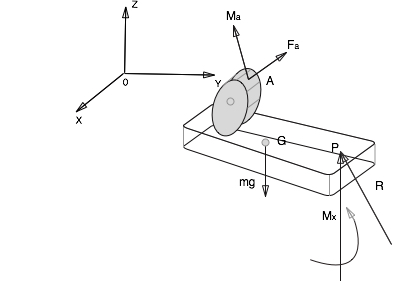
\includegraphics[width=0.7\textwidth]{1}}
			\caption{A sole with acting forces on it. mg is a gravity force. G is a center of gravity. P is a point of resulting ground reaction force application. R is a ground reaction force.}
			\label{fig:1}
			\vspace{-0.1cm}
		\end{figure}

		Figure \ref{fig:1} demonstrates only the sole separately from other parts of the leg. G is a Center of Gravity of the sole. At point P there is a resulting ground reaction. This ground reaction force maintains the robot in the equilibrium position. Equilibrium means that robot is not falling. The force of ground reaction R and moment M consists of its three components ($R_x$, $R_y$, $R_z$) and ($M_x$, $M_y$, $M_z$) respectively. Horizontal components of R should compensate friction force in the point of contact. Thus, the horizontal reaction of force ($R_x$, $R_y$) represents 
		friction force that compensate horizontal component of $F_a$. At the same time the moment $M_z$ represents friction reaction forces (see \cref{fig:2}).  It compensates vertical component of $M_a$ and the moment induced by $F_a$. \cite{vukobratovic2004zero}

		\begin{figure}[H]
			\vspace{-0.2cm}
			\centering
			{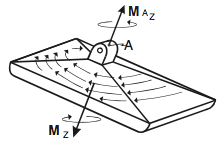
\includegraphics[width=0.7\textwidth]{2}}
			\caption{Rotational moment in the sole}
			\label{fig:2}
			\vspace{-0.1cm}
		\end{figure}

		 ZMP should lie in the foot plane in order robot to be stable \cite{kajita2003biped}. The problem is that we cannot manipulate the foot directly \cite{mitobe2000control}. According to \cite{vukobratovic2004zero} we can do it by ensuring the appropriate dynamics of the mechanism above the foot. If the resulting force in ZMP lies not in vertical direction (above mentioned conditions don't hold and thus R and $M_z$ didn't compensate correspondent components of $F_a$ and $M_a$) than the foot will slide. It means that dynamical stability was not achieved due to the fact, that there is a rotational moment which affects the robot. On the other hand, in \cite{sardain2004forces} it was proven that if ZMP lies in the foot area (that is usually called the support polygon) and moreover it coincides with the contact point with point P (see \cref{fig:1}), then the robot is stable, due to the fact, that all the resulting forces lie in the vertical direction. During the walk the position of ZMP should be computed continuously and the main problem of control is to keep ZMP and contact point to be coincided inside the support polygon of contact foot with the ground.
		The name zero moment point relates to the fact, that dynamical stability is maintained if horizontal components $M_x$ and $M_y$ are both equal to zero.
	
		\begin{equation}\label{eq:ZMP1}
			M_x = M_y = 0
		\end{equation}

		In the point P there should exist such equivalent force R and vertical moment $M_z$ that compensate the force reaction of the ground and maintain the stability of the construction. To achieve the dynamical stability the following equation should hold:

		\begin{equation}\label{eq:ZMP2}
			R + F_a + mg = 0
		\end{equation}

		Where $m$ is a mass of the foot and g is a gravitational acceleration. O is defined In \cite{vukobratovic2004zero} as the origin coordinates frame we can define radius vectors $\vec{OP}$, $\vec{OG}$ and $\vec{OA}$ where A is a point of ankle joint.

		\begin{equation}\label{eq:ZMP3}
			\vec{OP} \times \vec{R} + \vec{OG} \times mg + M_A + M_z + \vec{OA} \times F_a = 0
		\end{equation}

		Placing the origin frame at point P and making a projection on the horizontal plane gives us the following equations: 

		\begin{equation}\label{eq:ZMP4}
			(\vec{OP} \times \vec{R})^H + \vec{OG} \times mg + M_A^H + (\vec{OA} \times F_a)^H = 0
		\end{equation}
		
		Where H denotes horizontal component.\\
		
		Equation \ref{eq:ZMP4} represents the foot equilibrium \cite{vukobratovic2004zero}. However it doesn't solve the problem, because it is still unknown whether for the given motion of mechanism it (mechanism) is kept in the equilibrium. It is only if ZMP lies inside the support polygon.
		
		Thus, we have to make the following assumptions in order to compute the position of ZMP \cite{dekker2009zero}:

		\begin{enumerate}
			\item
				The bipedal robot consists of n rigid links.
			\item
				All kinematic information, such as position of Center of Mass (CoM), link orientation, velocities, etc. are known and calculated by forward kinematics.
			\item
				The floor is rigid and motionless.
			\item
				The feet cannot slide with regard to the floor surface.
			\item
				All joints are actively actuated.
		\end{enumerate}
	
		With this constraints we can define the mass of the robot as:
	
		\begin{equation}\label{eq:ZMP5}
			m_{robot} = \sum^n_{i=1}{m_i}
		\end{equation}

		Schematic bipedal robot with math m was considered in \cite{dekker2009zero} in order to derive the coordinates of ZMP (\cref{fig:3}).

		\begin{figure}[H]
			\vspace{-0.2cm}
			\centering
			{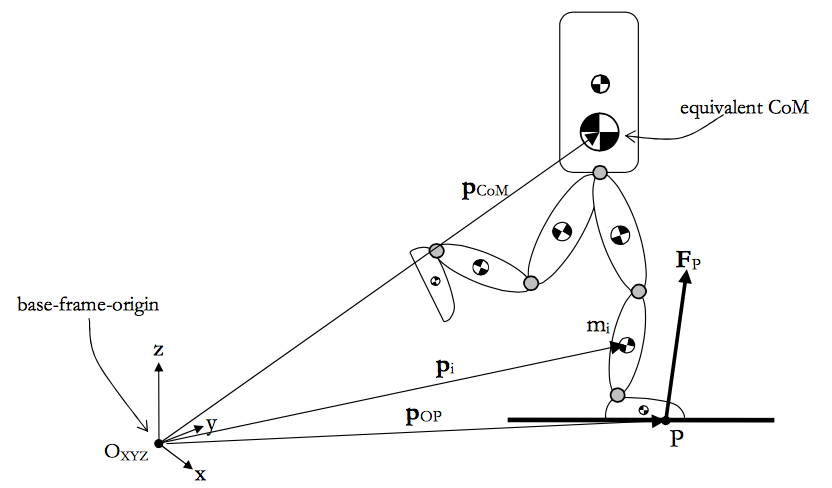
\includegraphics[width=0.7\textwidth]{3}}
			\caption{Rotational moment in the sole \cite{dekker2009zero}}
			\label{fig:3}
			\vspace{-0.1cm}
		\end{figure}

		$p_i$ are the distances between base frame and equivalent center of mass of i-link (see \cref{fig:3}). Then total linear momentum P given that $\dot{p_i}$ is $p_i$ velocity can be described by \ref{eq:ZMP6}.
	
		\begin{equation} \label{eq:ZMP6}
			P = \sum^n_{i=1}{m_i \dot{p_i}}
		\end{equation}
		And total angular momentum H is:
		\begin{equation} \label{eq:ZMP7}
			H = \sum^n_{i=1}{\dot{p_i} \times m_i \dot{p_i} + I_i \omega_i}
		\end{equation}

		where $\omega_i$ is an angular velocity and $I_i$ is inertia tensor of link i which is computed as:
		\begin{equation} \label{eq:ZMP8}
			I_i = R_i I_i^{\prime} R_i^T
		\end{equation}
		where $R_i$ is a rotation matrix that maps i-link coordinate frame w.r.t. the origin base frame, $R_i^T$ is transposed R and $I_i^{\prime}$ is a inertia matrix of i-link w.r.t. the link frame origin attached to their links.

		Taking the derivative of \ref{eq:ZMP6} and \ref{eq:ZMP7}:
		\begin{equation} \label{eq:ZMP9}
			\dot{P} = \sum^n_{i=1}{m_i \ddot{p_i}}
		\end{equation}
		\begin{equation} \label{eq:ZMP10}
			\dot{H} = \sum^n_{i=1}{\ddot{p_i} \times m_i \dot{p_i} + \dot{p_i} \times m_i \ddot{p_i} + I_i \dot{\omega_i}} + \omega_i \times I_i \omega_i
		\end{equation}

		where dots represents time derivatives.\\
		
		ZMP approach gives us the solution that is based on the principle of dynamical stability, however it is not energy efficient \cite{manchester2011stable}. It requires simultaneous control over all the joints of the robot. The method that was described in \cite{collins2001three} is called passive-walker dynamics and it uses gravity forces to reduce the amount of necessary energy to control the robot.\\
		
		In order not to loose the balance and not to fall active control of the robot should be performed with applying dynamical stability principle. So, it makes sense to apply passive-walker dynamics with ZMP based control.\\
		
		The most important task in the bipedal locomotion is to maintain dynamical stability \cite{vukobratovic2004zero}. It can be accomplished if the foot have a full contact with the ground, i.e. the contact is not only on the edge or at the point. Moreover it shows that ZMP position depends on the robot dynamics: the resulting force in the contact polygon and total moment in ZMP. So, during the motion the position of ZMP changes and there are situations when ZMP reaches the edge of a support polygon. In these situations if additional moments appear, robot will rotate around foot edge and will lose the stability. A way to measure the load on the sole is to analyze force sensors on it \cite{vukobratovic2004zero}. The algorithm of ZMP control is quite straightforward. Compute desired ZMP coordinates, measure the error between current ZMP position and reference ZMP value, apply correcting signal. A very important notion is Center of Pressure (CoP). As the pressure between foot and the ground can be replaced with the force applied in CoP \cite{vukobratovic2004zero}. With this we can define stability condition as ZMP and CoP coincidence. Usually ZMP is required to be under the center of the foot during a single support phase and moves to the other foot in the double support phase.\\
		ASIMO - a bipedal robot of Honda company, was build on top of this theory and the history of its evolution is described in \cite{hirai1998development}. Nowadays ASIMO is one of the most developed robots, it can interact with humans and perform different task  from playing footboll to stair climbing.\\ 
		In \cite{goswami1999postural} the problem of foot rotation was formulated. The author introduced the Foot-Rotation Indicator (FRI). FRI is the point, that can leave the support polygon. It describes the impeding rotation. When FRI lies outside the support polygon it means that there is rotational moment. In order to control instability of the gait acting on the foot is necessary to compensate this rotation.

	\section{Central Pattern Generator Approach}
		During the grows humans train the mechanism that can solve some simple problems without mental activities. This mechanism applies trained pattern to the problem. The name of this mechanism is reflex.
		An experiment conducted in \cite{grillner1975locomotion} shows that reflexes are significant for locomotion. During human brain reverse engineering a neural network that controls locomotion was found. It was situated in spinal regions which is the reason to name this network Central Pattern Generator (CPG).
		Another definition of CPG can be found in \cite{lee2007construction}: CPG is a rhythm generating network in the nervous system which creates and controls the rhythmic motor patterns of animal motions. CPG approach for gait generation was considered in \cite{miyakoshi1998three}. Neural oscillator was used for generation of motions for bipedal robot. Moreover it can be described as a neural network produces rhythmic pattern outputs without the need for patterned input \cite{wright2014intelligent}. CPG is a group of oscillating neurons with some phase between them which results into rhythmic body motion. The pattern is generated not only by the internal neural system but also by the external sensor information, e.g. info from sonar or camera \cite{miyakoshi1998three}. The key element in CPG is an adaptive neural element that can be described by a pair of first order differential equations. Each pair of the following equations forms an adaptive neuron.

		\begin{equation}\label{eq:CPG1}
			\tau_1 \dot{x}_1 = -x_1 - \beta f(\nu_1) -  \gamma f(x_2) + u_0 + u_{f_1}
		\end{equation}
		\begin{equation}\label{eq:CPG2}
			\tau_2 \dot{\nu}_1 = -\nu_1  + f(x_1)
		\end{equation}
		\begin{equation}\label{eq:CPG3}
			\tau_1 \dot{x}_2 = -x_2 - \beta f(\nu_2) -  \gamma f(x_1) + u_0 + u_{f_2}
		\end{equation}
		\begin{equation}\label{eq:CPG4}
			\tau_2 \dot{\nu}_2 = -\nu_2  + f(x_2)
		\end{equation}

		where $x_1$  is initial state of neuron, fired by the constant input $u_0$, $x_1$, $x_2$, $\nu_1$ and $\nu_2$ are state variables, dot represents time derivative.  When firing reaches some threshold, the neuron goes to state $\nu_1$ through eq. (\ref{eq:CPG2}). When it exceeds some threshold it starts to return to the state $x_1$ through the eq. (\ref{eq:CPG1}) by the factor $\beta$. $\beta$ represents the rate of adaptations, if $\beta$ is big, the return to state $x_1$ is fast. $u_{f_1}$ and $u_{f_2}$ are the feedback inputs from sensors, $\gamma$ is the coefficient between state variables and f(x) is a threshold function that has zero gain until x is less than threshold value and not zero gain otherwise . Such element works the following way: when it takes constant input it reacts, then adapts and stop reacting. Oscillations generation is the process of reaction and adaptation itself. \\
		
		Human like gait was achieved by a robot with small Degree of Freedom (DoF) in \cite{miyakoshi1998three}. The idea of this oscillator was to build a robust system that performs simple control with minimum structure of neural architecture that can be perspective for high DoF robot.\\
		
		A detailed examination of a biological CPG from an engineering perspective was conducted in \cite{zhu2006central} but, for most applications, the neuron pair is still approximated with a pair of differential equations \cite{wright2014intelligent}.

		These oscillators can be divided into two types : Simple Sinusoidal Oscillator and Systems of Differential Equations \cite{wright2014intelligent}, which are described in details bellow in Sec. 2.2.1 and Sec. 2.2.2

		\subsection{Simple Sinusoidal Oscillator}
			For a sinusoidal signal it is very easy to maintain phase relationships. Human sized bipedal robot controlled by Simple Sinusoidal Oscillator was considered in \cite{morimoto2008biologically}. The sinusoidal pattern is used for control of parameters, like phase or joint angle. The equation (\ref{eq:Sin1}) shows the example of hip angle control by phase $\phi$ and hip amplitude $A_{hip}$.
			\begin{equation}\label{eq:Sin1}
				\theta_{hip} (\phi) = A_{hip} sin(\phi) 
			\end{equation}
 			However it is a very simple model which is good for systems that are statically stable, but is not appropriate for anthropomorphic robots \cite{wright2014intelligent}. Statically stable systems are the systems that van maintain their stability during the continuous absence of movements.is good for systems that are statically stable
		\subsection{Systems of Differential Equations}
			Analysis of biological CPGs has identified that oscillators are made from pairs of mutually inhibiting neurons \cite{grillner1995neural}. These oscillators are applicable for the  generate different gaits and produce various solutions from sinusoidal to more complex forms. It can control anthropomorphic robot even on the rough terrain.
			\subsubsection{Matsuoka oscillator}
				Matsuoka oscillator is capable for different gaits and is widely used \cite{wright2014intelligent}. They are popular because of their dynamics and in particular limit cycle behavior \cite{matsuoka1985sustained}.
				
				The model of neuron with adaptation can be represented in the following way:
				\begin{equation}\label{eq:Mats1}
					\begin{split}
						\tau \dot{x} + x = \sum^n_{j = 1} c_j s_j - b x^{\prime}\\
						T \dot{x}^{\prime}  + x^{\prime} = y\\
						y = g(x - \theta)
					\end{split}
				\end{equation}
				
				Here $\tau$ is a variable, that represents time delay, $x$ is a membrane potential of the neuron, $s_j$ is an impulse rate of input stimuli, $\theta$ is a threshold value below which neuron doesn't fire, $c_j$ are weights of synaptic conjunctions ($>$ 0 for activating synapses and $<$ 0 for inhibitory synapses), y is a firing rate of the neuron, $x^{\prime}$ is the variable that represents the degree of the adaptation, T ($>$0) and b($\geq 0$) are parameters that specify the time course of the adaptation \cite{matsuoka1985sustained}.
				Activating synapses are neurons with positive signs of output signal.
				Inhibitory synapses are neurons that have negative sign of output signal.
				Degree of the adaptation is the speed of reaction to disturbance. Firing is the notion of process during which the neuron emits an action potential. 
				
				Matsuoka in \cite{matsuoka1985sustained} discusses oscillations generated by mutual inhibition between n neurons with adaptation:
				\begin{equation}\label{eq:Mats2}
					\begin{split}
						\dot{x}_i + x_i = - \sum^n_{j = 1} a_{ij} y_j - b x^{\prime} + s_i\\
						T \dot{x}^{\prime}_i  + x^{\prime}_i= y_i\\
						y = g(x_i)\ \ (i = 1,...,n) 
					\end{split}
				\end{equation}
				
				where $a_{ij}$ represents the strength of inhibitory connection between the neurons. $a_{ij} >$ 0 for i$\neq$j and $a_{ij}$ = 0 for i = j. $\sum^n_{j = 1} a_{ij} y_j $ is the total input from the neurons inside a neural network and $s_{i}$ is the total input from the outside of the network, $y_j$ is input from neuron j. 
				
				Matsuoka oscillator is schematically represented in \cref{fig:4}.
				\begin{figure}[H]
					\vspace{-0.2cm}
					\centering
					{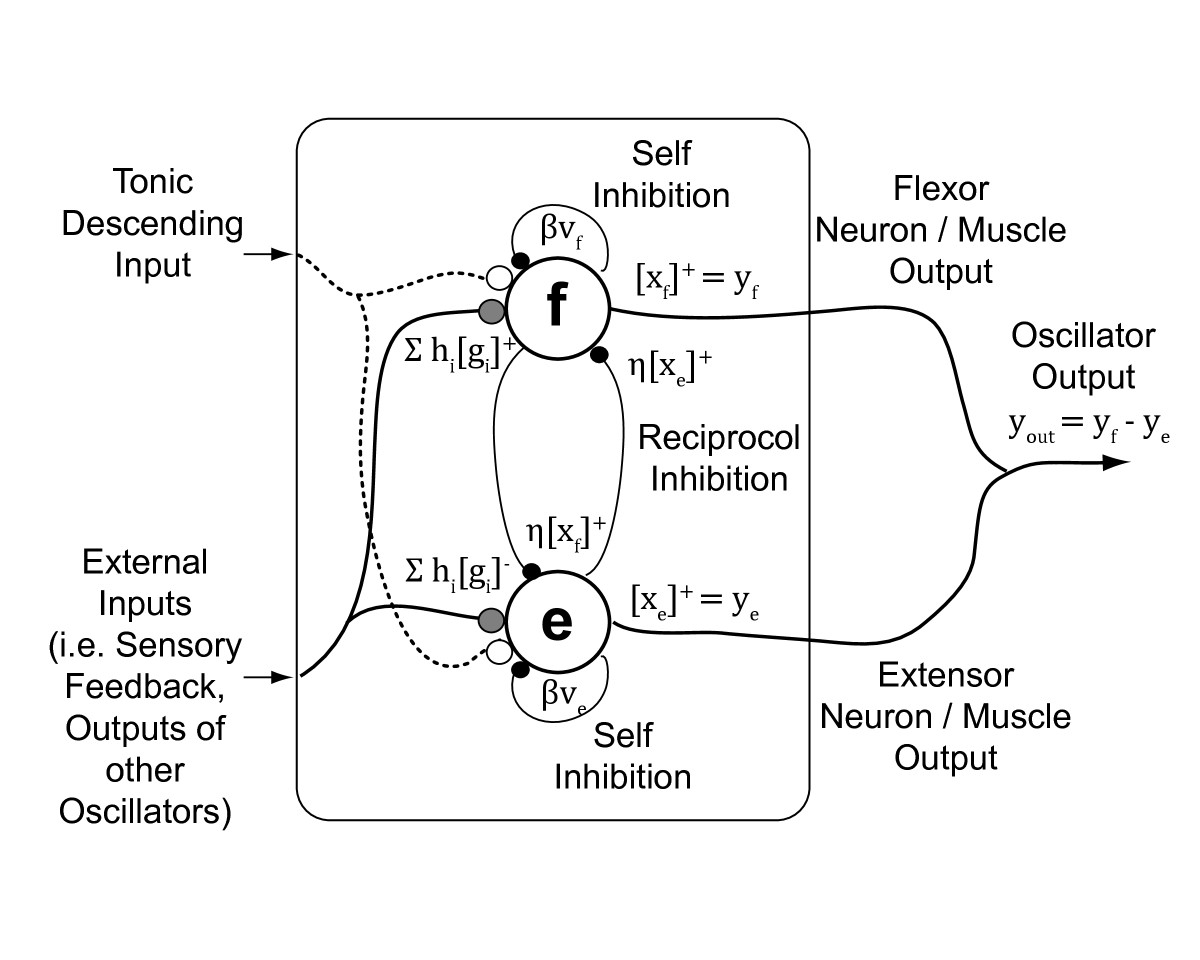
\includegraphics[width=0.7\textwidth]{4}}
					\caption{Matsuoka oscillator \cite{liu2008central}}
					\label{fig:4}
					\vspace{-0.1cm}
				\end{figure}
				
				Two neurons, a flexor (f) and an extensor (e), reciprocally inhibit each other. External inputs ($g_i$) such as sensory feedback or inputs for other neurons can be either inhibitory or excitatory, depending on the gain ($h_i$) - that is defined by external sensory inputs. Black circles indicate inhibitory inputs. White circles indicate excitatory inputs. Gray circles can be either inhibitory or excitatory.
			\subsubsection{Van der Pol oscillator}
				Van der Pol oscillator benefits are stable limit cycles and relatively interpretable coefficients. Frequency, amplitude and shape coefficients can be identified, although they are not completely independent. Transition between gaits is reached with a simple change of oscillator parameters.
				
				The equation of Van der Pol oscillator is:
				
				\begin{equation}\label{eq:Pol1}
					\ddot{x} - \epsilon(1 - x^2)\dot{x} + x = 0
				\end{equation}
				
				where x is the dynamical variable and $\epsilon > 0$ a parameter, a dot represents time derivative.
				The van der Pol oscillator has exactly one limit cycle and all other trajectories spiral into it which is proved in \cite{kanamaru2007van}.
			\subsubsection{Rayleigh oscillator}
				Rayleigh oscillator is similar to the Van der Pol oscillator but it has reduced sensory requirements, that is an advantage over conventional prosthetic systems.
				
				The equation of Rayleigh oscillator is:
				
				\begin{equation}\label{eq:Rel1}
					\ddot{x} + \epsilon(3x^2 - 1)\dot{x} + (\omega^2 - \epsilon)x = 0
				\end{equation}
				
				where x is the dynamical variable and $\epsilon > 0$ a parameter, a dot represents time derivative.
				Comparison of \ref{eq:Rel1} and \ref{eq:Pol1} shows that Rayleigh oscillator is parametrized with $\omega$ Van der Pol oscillator.
			\subsubsection{Spiking Integrate and Fire with Adaption neurons}
				Spiking Integrate and Fire with Adaption neurons were used in \cite{russell2007configuring} for bipedal locomotion. The CPG has a hierarchical structure of hip timing, knee timing and output patterning. This structure allowed to tune parameters of every of three hierarchical parts, and so to configure walking frequency, gait and joint angles independently.
		\section{Neural Networks Approach}
		Despite the fact that oscillators can be described as a neural network they do not require any input for their work. Canonical Neural Networks (NN) have input data and output. There are several groups of NN that are used for bipedal robots control. The most popular of them are described bellow.

			\subsection{Feed-Forward Networks}
				In this networks each neuron has its own connection and transfer function. Feed-Forward Networks are ready for state motion generation.  Input data is current kinematics and sensory data. Current kinematics is the kinematic configuration in the given time frame. 
				\subsubsection{Multi-layer Perceptron}
					Multi-layer perceptron (MLP) is one of such models. They can have three (input, output, hidden) and more layers (more hidden layers). According to \cite{vundavilli2010dynamically}, two MLPs were used to specify parameters of a bipedal ditch crossing gait trained with Genetic Algorithm (GA). It produced the best solution in terms of stability. It was more stable and efficient than one from a fully analytical approach, and slightly better than the result obtained with a fuzzy logic based method.
				\subsubsection{Radial Basis Function Network}
					Radial Basis Function Network is another example of Feed-Forward Networks (FFN). Activation function is usually Gaussian (\ref{eq:gf}) or Euclidean which is described in \cite{EuclideanFunction}.
					
					\begin{equation}\label{eq:gf}
						f(x) = a exp \left(  - \dfrac{(x - b)^2}{2c^2} \right)
					\end{equation}
					
					Neurons in hidden layers are connected only with a small part of input neurons. For this reason two types of vectors are necessary: wights vector and centre vector (centre vector dimension is the same as input one). Each vector responds if it is close to the weights vector. Output neurons are functions of linear combinations of network outputs and their wighted connections.
					It was successfully used for hexapod locomotion \cite{ilg1995learning}.
				\subsubsection{Cerebellar Model Articulation Controller}
					A Cerebellar Model Articulation Controller (CMAC) is a type of associative memory network based on cerebellum \cite{albus1975new}. Input space is continuous and divided into hyper-rectangles. So input should be located in one rectangle at each moment. Numerous hidden layers are stored in slightly moved from the input rectangles. Hence rectangles will overlap on different layers. The output for each layer is a weighted sum of activated rectangles. Activated rectangle is one that are placed near the input point. The CMACs successfully learned the movement patterns and showed resilience to perturbations (including uneven or slippery floors), thereby translating a rigid analytical solution into an adaptable one \cite{sabourin2005robustness}.
			\subsection{Recurrent Networks}
				The structure of such networks is more complicated that FFN. Thus we can produce more complex patterns and handle different types of input.
				
				For recurrent networks there are different types of input and the difference from FFN is that pattern is not required to be provided as an input but it is generated , tuned or chosen internally by the inputs. 
				
				\subsubsection{Jordan and Elman Recurrent Neural Networks}
					Jordan recurrent NN is similar to FFN, the difference is that output of the network is recurrently fed to the input.\\
					The example of Elman recurrent NN is shown in (\cref{fig:5}). The difference between Elman recurrent NN and Jordan recurrent NN is that delayed output of hidden layer $y_i$ is connected with the inputs of a hidden layer. A delay here is done by $u_i$ nodes from the hidden layer. The Elman network was used in \cite{berns1995neural}, the resilient back-propagation training algorithm was used and the system showed an ability to learn supervised trajectories and interpolate between them.
					
					\begin{figure}[H]
						\vspace{-0.2cm}
						\centering
						\scalebox {0.7} {
							\begin{tikzpicture}[ -,>=stealth',shorten >=1pt,auto,node distance=3cm,
								thick,main node/.style={circle,draw,font=\sffamily\Large\bfseries}]
								
								\node (1) {};
								\node[main node] (2) [right of=1] {$x_1$};
								\node[main node] (3) [right of=2] {$y_1$};
								\node[main node] (4) [right of=3] {$z_1$};
								\node (5) [right of=4] {$b_1$};
								\node (6) [below of=1] {};
								\node[main node] (7) [below of=2] {$x_2$};
								\node[main node] (8) [right of=7] {$y_2$};
								\node[main node] (9) [right of=8] {$z_2$};
								\node (10) [right of=9] {$b_2$};
								\node (11) [below of=6] {};
								\node[main node] (12) [below of=7] {$x_n$};
								\node[main node] (13) [right of=12] {$y_n$};
								\node[main node] (14) [right of=13] {$z_n$};
								\node (15) [right of=14] {$b_n$};
								\node[main node] (16) [below of=13] {$u_1$};
								\node[main node] (17) [below of=16] {$u_2$};
								\node[main node] (18) [below of=17] {$u_3$};
								
								\path[every node/.style={font=\sffamily\small}]
							    	(1) edge node {$in_1$} (2)
									(2) edge node {$w_{x_1y_1}$} (3)
								         edge node {} (8)
								         edge node {} (13)
								    (3) edge node {$w_{y_1z_1}$} (4)
										 edge node {} (9)
										 edge node {} (14)
								    (6) edge node {$in_2$} (7)
								    (7) edge node {} (3)
										 edge node {} (8)
										 edge node {} (13)
									(8) edge node {} (4)
									     edge node {} (9)
									     edge node {} (14)
									(11) edge node {$in_n$} (12)
									(12) edge node {} (13)
									       edge node {} (8)
									       edge node {} (3)
									(13) edge node {} (14)
									       edge node {} (9)
									       edge node {} (4);
								\path[->, every node/.style={font=\sffamily\small}]
							  	    (3) edge [bend left] node[right] {} (16)
							  	    (8) edge [bend left] node[right] {} (17)
							  	    (13) edge [bend left] node[right] {} (18)
									(4) edge node {} (5)
									(9)	edge node {} (10)
	                                (14) edge node {} (15)
	                                (16) edge [bend left] node[right] {} (3)
	                                (17) edge [bend left] node[right] {} (8)
	                                (18) edge [bend left] node[right] {} (13);
	                             \path[draw=white]
		                             (7) edge node {$\vdots$} (12)
		                             (8) edge node {$\vdots$} (13)
		                             (9) edge node {$\vdots$} (14)
		                             (17) edge node {$\vdots$} (18);
							\end{tikzpicture}
						}
						\caption{Elman recurrent NN. Inputs are $x_i$, hidden layer contains nodes $u_i$ that delays connected to them outputs of $y_i$. Outputs of the network are nodes $Z_i$}
						\label{fig:5}
						\vspace{-0.1cm}
					\end{figure}
					
				\subsubsection{Fully Connected Recurrent Neural Networks}
					In several works \cite{reil2002evolution}, \cite{petridis1994recurrent} a network of several fully connected leaky-integrator neurons were used as a pattern generator. 
					
					The network was able to learn multiple sinusoidal patterns, selectable by an input level, but evolution took more generations as the number of required patterns increased. Learned patterns were resilient to noise at the inputs, and even if the input was disrupted by a large amount, the output would quickly return to normal when the input was corrected. It was found that a six neuron model was sufficient to store eight different sinusoidal patterns, as long as the form of those patterns was different \cite{wright2014intelligent}.
					
					The problem of GA parameters optimization is that for complex systems a huge amount of generations will be necessary. So it can be applied only for offline patterns generation. 
				\subsubsection{Reservoir}
					Usually recurrent NN should be as small as possible in order to simplify parameters tuning. Reservoir network follows a different principle. It uses a big network with potentially much redundancy. The idea is that during training only output layer is trained and reservoir is unchanged. It works with the following assumption: system dynamics is already present when the network is constructed randomly and the only necessary thing is to adjust weights for it. Thus the training process is very simple, e.g. a linear regression.
					
					Generating trajectories with reservoir can be done taken the human captured data as input \cite{wyffels2009design}.
		\section{Hidden Markov Model Approach}
			Learning by imitation is one of commonly used approaches for bipedal locomotion researches. Obviously, direct copying of movements of an operator is impossible due to different kinematic and dynamic characteristics. So, from the operator we can take only the pattern and then imitate it on the robot. Observing here is estimating the underlying state variables. It is based on the source system through the output data. For this task Hidden Markov Models (HMM) can be used \cite{inamura2004embodied}. 
			
			A recognition algorithm is used for identification of movement. If movement was not identified, it is added to the database as new. Hidden Markov model provides abstraction of the pattern which is used for motion synthesis. Although typically used for imitation tasks, HMM have also been employed to detect problematic states.	HMM itself is a finite state automaton. It is defined by a set of states with initial and final states, transition probability matrix where element $a_{ij}$ is the probability of transition from state i to state j.
			
			 Controller basing on its input generates an output signal that is called the control signal. Input for controller is difference between reference signal and system output. In order to obtain a finite set of decision patterns, it is necessary to divide the control space into a finite number of subspaces. According to  \cite{yang1994hidden}, the following steps are necessary to define an HMM-based controller:
			
			\begin{enumerate}
				\item
					A correspondence  between the control signal and controller input (error signal) can be established due to the definition of HMM the control signal depends only on a finite number of previous input signals.
				\item 
					Define a set of patterns. At each time the control signal belongs to one of the patterns. Also control signal at each moment of time corresponds to one of the set of k previous input signals.
				\item
					It is necessary to label the data. It means that the set of input signals is mapped to the set of possible control signals.
				\item
					Train the model by the data describing control signals.
				\item
					Collect a set of trained models.
			\end{enumerate} 
			
			HMM are good for simple systems control, however it requires a lot of space and time for teaching the HMM controller to work with complex multi body systems.
			
		\section{Rule Based Approach}
			After the identification of the current state we can find the next one using rule-based method. For bipedal robots fuzzy-logic systems were used in some researches \cite{park2003fuzzy}.  A fuzzy logic controller helps to deal with a bit of uncertainty in the environment. And it can be used to vary ZMP position in the support polygon \cite{park2003fuzzy}. For the work it requires optimization of rules, that were basically chosen \cite{vundavilli2010dynamically}.
			The main idea is to divide the set of all possible system configurations into the clusters. For each cluster assign the control function. Hence during the work control function will be chosen according to the current robot configuration from the set of all possible control functions according to the current configuration.
			Fuzzy logic controller is a  perspective approach for solving dynamical stability problem for bipedal robots because it divide all the configuration space into the subspaces. For each subspace control function is  defined in an optimal way.
		
	\chapter{Bipedal Locomotion Control}
		According to the literature review there are a lot of different approaches for bipedal robot locomotion. In this work several of them were combined.
		We define two support phases of walking: single support phase (during this phase only one foot is in contact with the ground) and double support phase (two feet are in the contact ground simultaneously).
		
		\section{Locomotion Phases}
			We can break bipedal locomotion into the following phases \cite{rostami1998impactless}:
			
			\begin{enumerate}
				\item Stance phase.\\
					During this phase the load is on a bearing leg. It starts from the double support phase during weight acceptance. Than during single limb support phase only bearing leg is in the contact with the ground.
				\item Swing phase.\\
					During this phase there is limb advancement. It starts from double support phase and than finishes with single support phase.
			\end{enumerate}
			
			This phases can be identified on (\cref{fig:26}).
			 \begin{figure}[H]
			 	\vspace{-0.2cm}
			 	\centering
			 	{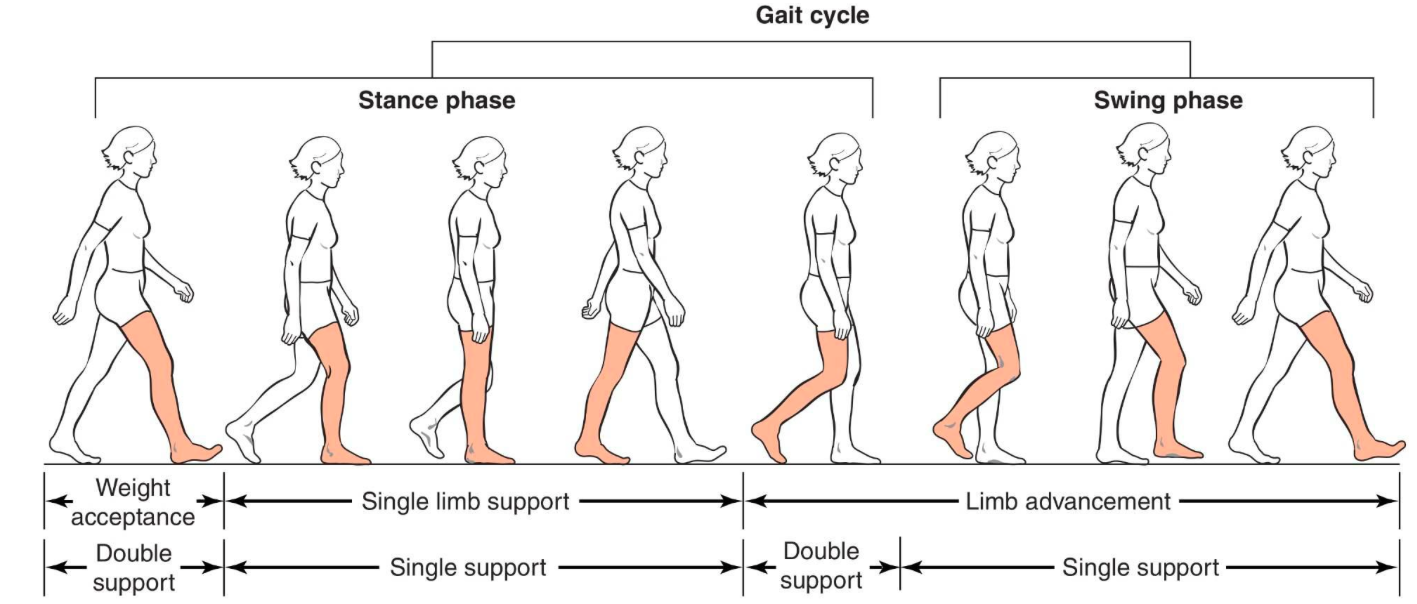
\includegraphics[width=1\textwidth]{26}}
			 	\caption{Human gait cycle \cite{gait}}
			 	\label{fig:26}
			 	\vspace{-0.1cm}
			 \end{figure}
			
		\section{Human Locomotion Models}
			One of the most simple models of human during single support phase is cart-table model, which is represented in \cref{fig:6}.
			
			\begin{figure}[H]
				\vspace{-0.2cm}
				\centering
				{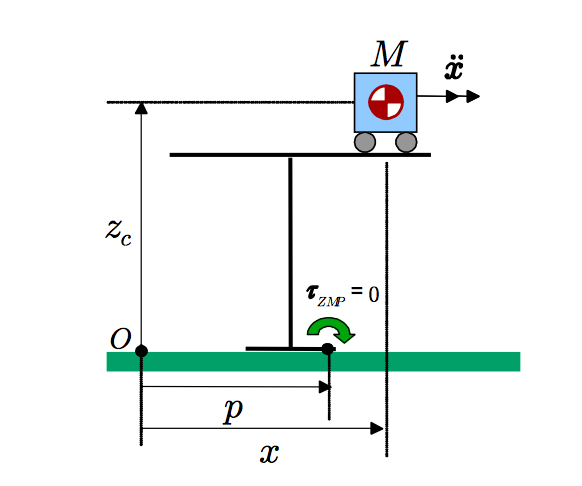
\includegraphics[width=0.7\textwidth]{6}}
				\caption{Cart-table model \cite{kajita2003biped}. M is cart mass. $Z_c$ is the height of cart CoM. $\tau_{ZMP}$ is the moment around ZMP. x is the cart trajectory, $\ddot{x}$ is the cart acceleration}
				\label{fig:6}
				\vspace{-0.1cm}
			\end{figure}
			
			When cart is far away from the Center of Mass (CoM), ZMP point goes out of support area shown in \cref{fig:6}. When it happens the system becomes unstable. The distance from zero point O to the center of table support polygon is denoted as X, the distance from zero to ZMP coordinate is denoted as P.
			The equation that describes this process was derived in \cite{kajita2003biped} and is represented bellow:
			
			\begin{equation}\label{eq:eqv1}
				P = x -\dfrac{Z_c}{g} \ddot{x}
			\end{equation}
			
			where $Z_c$ is the height of CoM of the cart, g is the gravitational acceleration and $\ddot{X}$ is the second time derivative.\\
			In order to prevent system falling we have to control the cart in the way that maintains the trajectory of ZMP of the system which guaranties that ZMP always stays inside the support polygon. When ZMP lies within the support polygon it maintains the dynamical stability of the system. When it leaves the region of support polygon we have a risk that the system can loose the stability and fall. Thus our target is to define the desired ZMP trajectory of the system. We define two planes in which the robot can move: frontal and sagittal planes. Also while there exists a transverse plane as well. We now consider only locomotion in frontal plane for simplicity. All the planes are represented in \cref{fig:7}. Desired trajectory for our system in frontal plane is provided in \cref{fig:8}.
			
			\begin{figure}[H]
				\vspace{-0.2cm}
				\centering
				{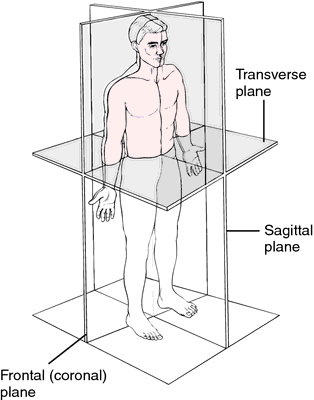
\includegraphics[width=0.4\textwidth]{7}}
				\caption{Human planes \cite{medical}}
				\label{fig:7}
				\vspace{-0.1cm}
			\end{figure}
			\begin{figure}[H]
				\vspace{-0.2cm}
				\centering
				{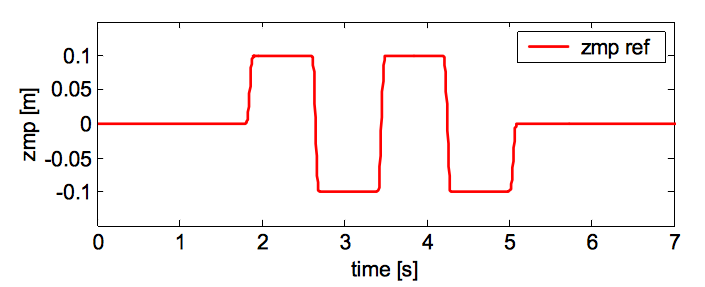
\includegraphics[width=0.8\textwidth]{8}}
				\caption{Desired ZMP trajectory in frontal plane \cite{kajita2003biped}. ZMP reference is the desired ZMP trajectory. ZMP is measured from zero in frontal plane.}
				\label{fig:8}
				\vspace{-0.1cm}
			\end{figure}
			Desired trajectory represents the movement of ZMP from the region of standing foot to the region of swinging foot in the moment of the step completing. Here the amplitude of frictions is defined by parameters of robot (step width in frontal plane). Thus we can build a simple control system represented in \cref{fig:9}. The input of this system is the reference trajectory of ZMP. Controller takes the error between reference ZMP trajectory and real measured ZMP trajectory as an input and generates control signal that is applied to the cart. 
			\begin{figure}[H]
				\vspace{-0.2cm}
				\centering
				{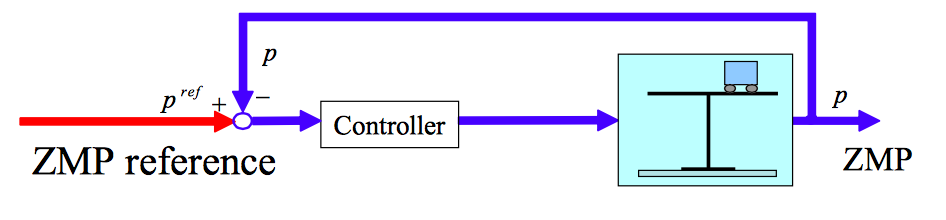
\includegraphics[width=0.7\textwidth]{9}}
				\caption{PID regulated ZMP control \cite{kajita2003biped}}
				\label{fig:9}
				\vspace{-0.1cm}
			\end{figure}
			If the controller is PID (proportional integral derivative) the regulator which maintains ZMP trajectory close to the desired one. We can see in \cref{fig:10} that our real ZMP trajectory follow the desired trajectory with the late. The result of such control is represented in \cref{fig:10}.
			\begin{figure}[H]
				\vspace{-0.2cm}
				\centering
				{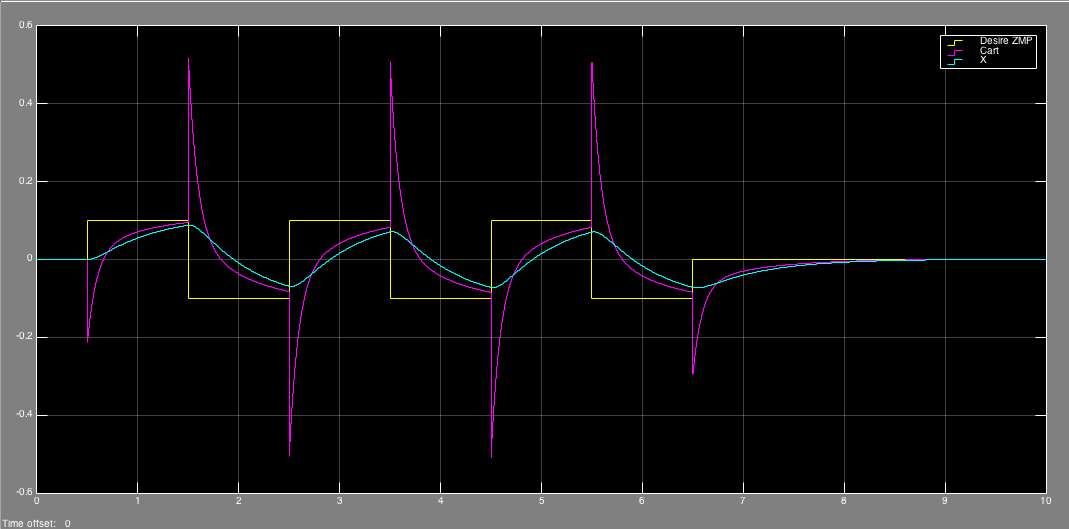
\includegraphics[width=1\textwidth]{10}}
				\caption{PID regulated ZMP trajectories. Due to fast change of desired trajectory in the moment of phase change real ZMP trajectory the fast risings.}
				\label{fig:10}
				\vspace{-0.1cm}
			\end{figure}
			Kajita et all in \cite{kajita2003biped} introduced a simple idea, to look forward to the desired ZMP  and try to predict what will happen before it happens. Hence the theory of optimal control comes into view and it will be described bellow how to make a predictive control system for such an unstable object as cart on the table model. Further Chapter 4 presents such controller being applied to the model of a biped robot and than demonstrates the evaluation of it.
			
		\section{Optimal Control}
			Next we introduce a discrete-time state-space model. Equation \ref{eq:oc1} introduces this model. This system of equations represents a dependency between the next state and current state of system though variables x and y \cite{hazell2008discrete}.
			
			\begin{equation}\label{eq:oc1}
				\begin{split}
					x(k+1) = Ax(k) + Bu(k)\\
					y(k) = Cx(k) + Du(k)
				\end{split}
			\end{equation}
			
			Where k is a discrete time index, x(k) is a vector of state values (trajectory, velocity and acceleration), u(k) is a control signal (jerk), y(k) is a vector of system output values (trajectory, velocity and acceleration). A, B, C, D are  appropriately dimensioned real matrices that defines system parameters and would be defined further in this chapter \cite{hazell2008discrete}.
			
			We define G, the  transfer function associated with model defined be eq. (\ref{eq:oc1}). G is defined as in \ref{eq:oc2}
			
			\begin{equation}\label{eq:oc2}
				G(Z) = C(ZI - A)^{-1}B+D
			\end{equation}
			
			Where Z is Z-transform variable and I is an identity matrix.
			
			We can estimate the size of the transfer function by measures $H_2$ and $H_\infty$. $H_2$ norm will be denoted as $||G(Z)||_2$ and is defined as in the following way:
			
			\begin{equation}\label{eq:oc3}
				||G(Z)||_2 = Tr\{ B^{T} XB + D^{T} D \}
			\end{equation}
			
			Where $X$ should satisfy eq. (\ref{eq:oc4}).
			
			\begin{equation}\label{eq:oc4}
				X = A^{T} XA + C^{T} C
			\end{equation}
			
			$H_2$ norm of the transfer function is a gain in power from input to output, assuming that the input signal is white \cite{hazell2008discrete}.

			$H_\infty$ is denoted as $||G(Z)||_\infty$ and is defined as:
			
			\begin{equation}\label{eq:oc5}
				||G(Z)||_\infty = \sup_{\omega} \dfrac{||z||_2}{||\omega||_2}
			\end{equation}
			
			where $z = G\omega$, $\omega$ is assumed to be a realization of a unit power, Gaussian, white-noise process and z is the real values vector of input. Hence $H_\infty$ defines the maximum possible gain in power from input ot output.
			
			\begin{figure}[H]
				\vspace{-0.2cm}
				\centering
				{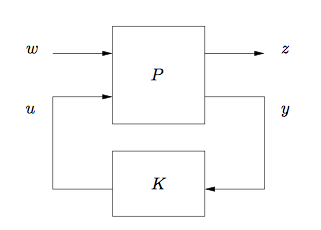
\includegraphics[width=0.5\textwidth]{11}}
				\caption{Generalized regulator \cite{hazell2008discrete}}
				\label{fig:11}
				\vspace{-0.1cm}
			\end{figure}
			
			There is a generalized regulator in \cref{fig:11}. The input for the system is $\omega$. The system is controlled by input signal u, $\omega$ represents all exogenous inputs including noise and disturbances. The system returns an output signal z, while y is measurements and references output. Thus K here is a feedback controller and P represents the controlled system.
			
			The following matrix equation
			
			\begin{equation}\label{eq:oc6}
				X = A^{T}XA + Q - \bar{L}^{T} \bar{R}^{-1} \bar{L}
			\end{equation}
			
			is known as Discrete Algebraic Riccati Equation (DARE). Here $\bar{R} = R + B^{T}XB$ and $\bar{L} = L + B^{T}XA$. The solution of this equation derived in \cite{hazell2008discrete}. Also we can write DARE in a short form: $X = D(A,B,Q,R,L;X)$ and $D(A,B,Q,R,L;X) = A^{T} XA + Q -  \bar{L}^{T} \bar{R}^{-1} \bar{L}$.
		
		\section{Preview Control} 
			Katayama et al. in \cite{katayama1985design} introduced a new method of control for general regulators with preview control. The key idea was to look forward for N discrete steps and predict the desirable value of controlled signal. The form of the control signal was derived as a theorem in \cite{katayama1985design}. The theorem says that the optimal control signal have the form of:
			
			\begin{equation}\label{eq:pc1}
				u(k) = -G_I \sum^{k}_{i=0} e(i) - G_xx(k) - \sum^{N}_{l=1}G_d(l)y_d(k+l)
			\end{equation}
			
			Where $G_I = [R+\tilde{B}^T \tilde{K} \tilde{B}]^{-1} \tilde{B}^T \tilde{K} \tilde{I}$ represents integral coefficient, e(i) is an error between controlled value and its referenced value, $G_x = [R+\tilde{B}^T \tilde{K} \tilde{B}]^{-1} \tilde{B}^T \tilde{K} \tilde{F}$ represents proportional coefficient, x(k) is the controlled value, $G_d(1) = -G_I$ and $G_d(l) = [R+\tilde{B}^T \tilde{K} \tilde{B}]^{-1} \tilde{B}^T \tilde{X}(l-1)$ represents feature coefficients at time l, $y_d(t)$ is a value of reference signal at time t.
			
			with the solution of DARE $\tilde{K}$ in the form:
			
			\begin{equation}\label{eq:pc2}
				\tilde{K} = \tilde{A}^T\tilde{K}\tilde{A} - \tilde{A}^T \tilde{K} \tilde{B} [R + \tilde{B}^T \tilde{K} \tilde{B}]^{-1} \tilde{B}^T\tilde{K}\tilde{A} + \tilde{Q}
			\end{equation}
			
			where:
			
			\begin{equation}\label{eq:pc3}
				\tilde{B} = \begin{bmatrix} C B \\ B \end{bmatrix},
				\tilde{I} = \begin{bmatrix} I_p \\ 0 \end{bmatrix},
				\tilde{F} = \begin{bmatrix} CA \\ A \end{bmatrix},
				\tilde{Q} = \begin{bmatrix} Q_e & 0 \\ 0 & Q_x \end{bmatrix},
				\tilde{A} = \begin{bmatrix} \tilde{I} & \tilde{F} \end{bmatrix}
			\end{equation}
			
			And finally $I_p$ is a $p * p$ identity matrix p is defined by the size of matrices C and A in order to allow computation of matrix $\tilde{A}$.
			
			Kajita et al. in \cite{kajita2003biped} proved that the necessary prediction for the cart table model is 1.6 seconds due to the dependency law on this parameter which is shown in \cref{fig:12} 
			
			\begin{figure}[H]
				\vspace{-0.2cm}
				\centering
				{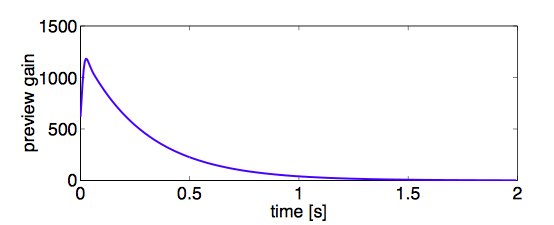
\includegraphics[width=0.7\textwidth]{12}}
				\caption{Power Gain dependency from the time \cite{kajita2003biped}}
				\label{fig:12}
				\vspace{-0.1cm}
			\end{figure}
			
			For the moment we have everything to design control system for the model of bipedal robot.
	\chapter{Implementation And Evaluation}
		The modeling of real-world objects is a very difficult task. It takes into account physical lows, gravity and frictions. Simulation environment for this thesis is Simulink.  Simulink is a framework in matlab environment. It provides primitives that can be used for real world models building. Also it provides the interface for high-level frameworks, that realizes high-level primitives for modeling. SimMechanics is one of packages in Simulink. It contains the blocks for mechanical modeling of multi body systems.  Robots are multi body systems and hence SimMechanics is a suitable choice for the environment.
		
		\section{Cart Table Model}
			Initially the cart table model was developed. The design is represented in \cref{fig:13}
			\begin{figure}[H]
				\vspace{-0.2cm}
				\centering
				{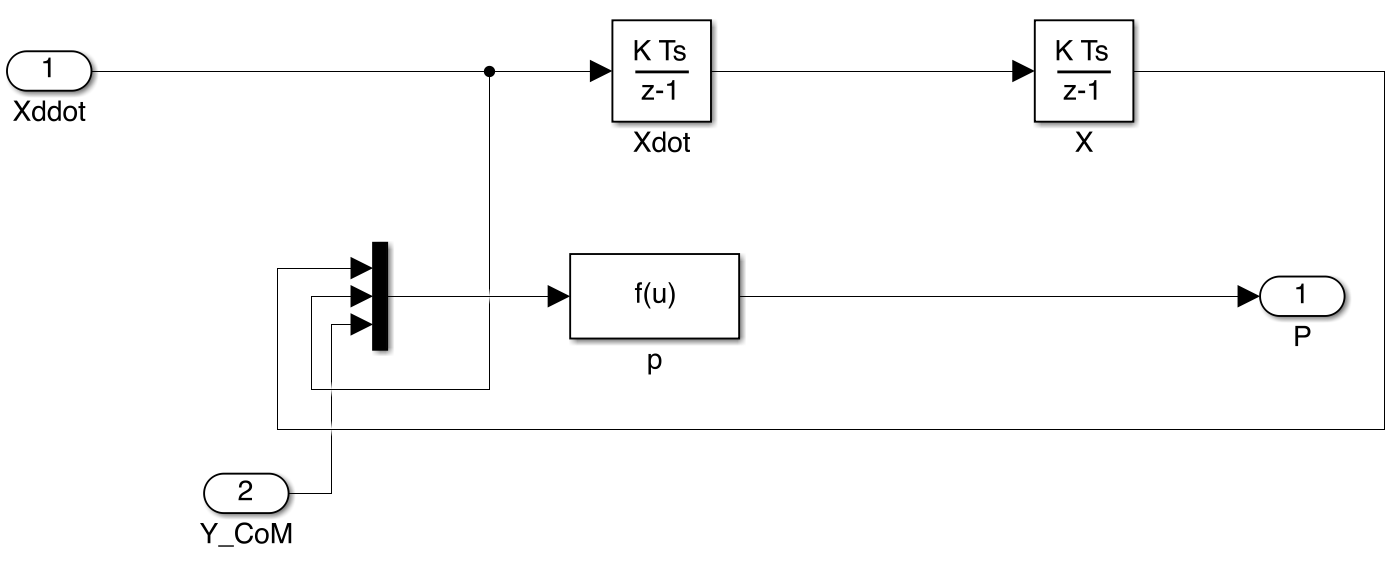
\includegraphics[width=1\textwidth]{13}}
				\caption{Cart-table model. Xddot is acceleration, Xdot is velocity, X is trajectory of cart CoM. Y\_CoM is the height of cart CoM. P is computed ZMP position.}
				\label{fig:13}
				\vspace{-0.1cm}
			\end{figure}
			
			Further it will be represented as a block on \cref{fig:14}.
			
			\begin{figure}[H]
				\vspace{-0.2cm}
				\centering
				{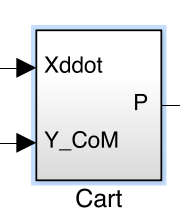
\includegraphics[width=0.2\textwidth]{14}}
				\caption{Cart-table model block. Xddot is second time derivative of the input (velocity of CoM). Y\_COM is the height of CoM that can deviate and thus cannot be constant. P is a computed cart's ZMP trajectory.}
				\label{fig:14}
				\vspace{-0.1cm}
			\end{figure}
			
			\subsection{PID Controller}
				This system is controlled by the second time derivative that represents speed. For the initial control model Proportional Integral Derivative (PID) regulator was applied. The system of PID regulated cart-table model is shown in \cref{fig:15}.
				
				\begin{figure}[H]
					\vspace{-0.2cm}
					\centering
					{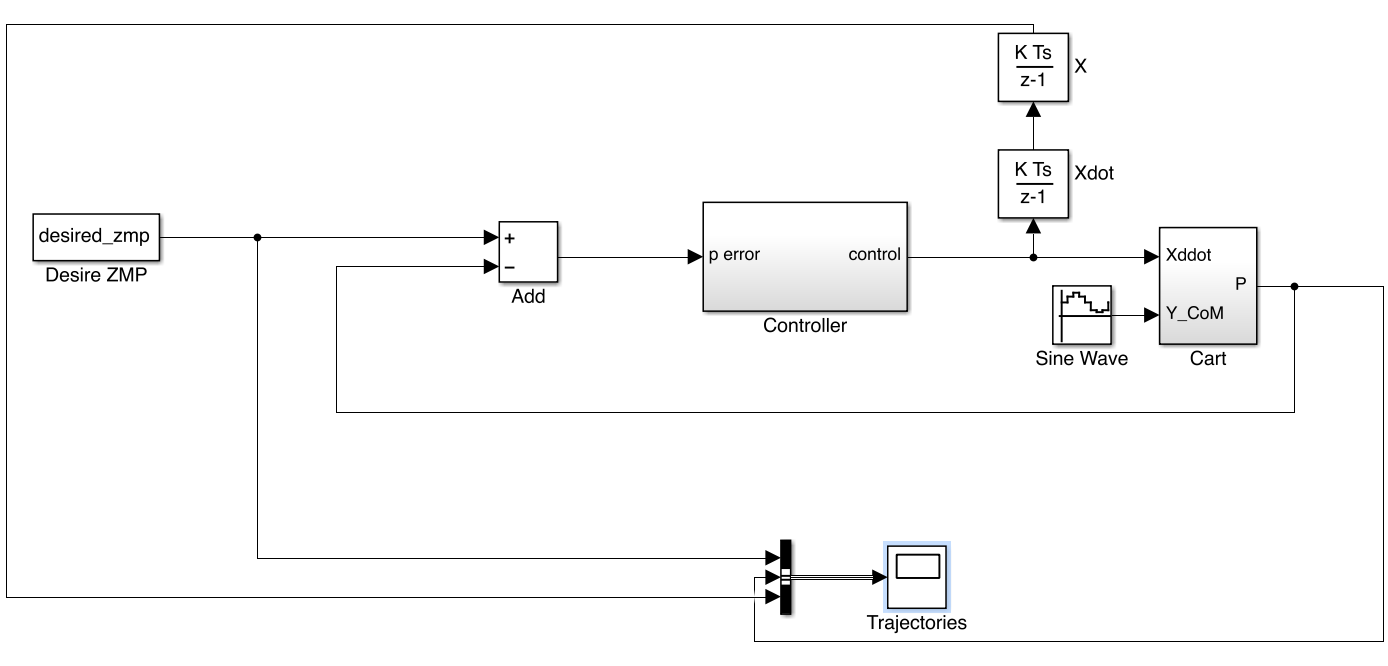
\includegraphics[width=1\textwidth]{15}}
					\caption{PID regulated cart-table. X is trajectory of CoM. Desired ZMP is reference ZMP trajectory. P is real measured ZMP trajectory. Xdot is a velocity, X is trajectory of a cart. Sine wave with low amplitude was used for modeling cart CoM height}
					\label{fig:15}
					\vspace{-0.1cm}
				\end{figure}
				
				The regulator is demonstrated in \cref{fig:16}.
				
				\begin{figure}[H]
					\vspace{-0.2cm}
					\centering
					{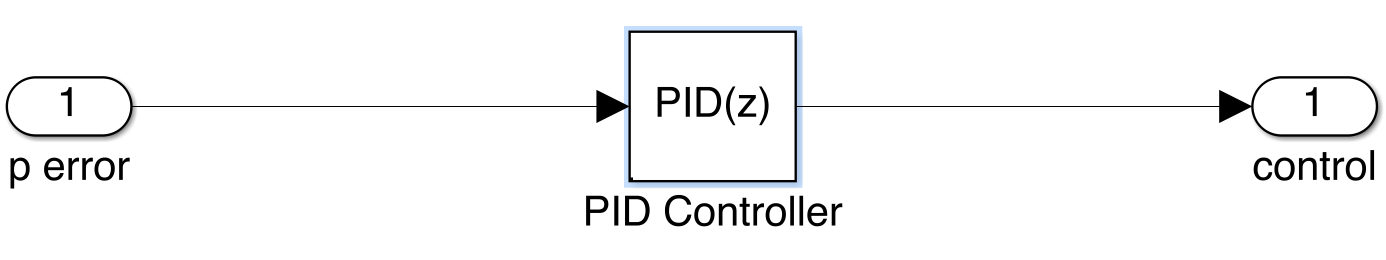
\includegraphics[width=0.7\textwidth]{16}}
					\caption{PID controller. P error is the error between reference ZMP and measured ZMP. Control is velocity of cart table model that is necessary to compensate the error between desired ZMP and measured ZMP.}
					\label{fig:16}
					\vspace{-0.1cm}
				\end{figure}
				
				The results of such control are represented on \cref{fig:17}.
				
				\begin{figure}[H]
					\vspace{-0.2cm}
					\centering
					{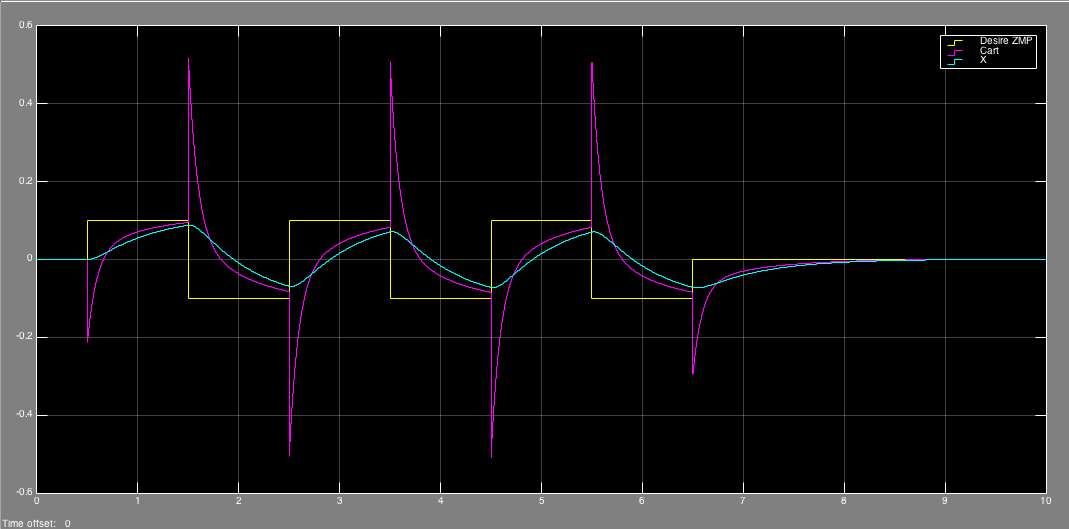
\includegraphics[width=1\textwidth]{17}}
					\caption{PID regulator control results. Desired ZMP is yellow and it is a reference signal for ZMP. Cart ZMP is violet and it represents measured value of cart ZMP. CoM trajectory is blue. Over control is observed because of PID transfer function impacts system stability.}
					\label{fig:17}
					\vspace{-0.1cm}
				\end{figure}
				
				We can see that the actual ZMP trajectory lates and due to this fact the CoM trajectory reaches the bound of support polygon and thus it makes the system unstable.
			
			\subsection{Preview Controller}
				After that the preview control with 1.6 second prediction was applied. The model of preview controller  is represented in \cref{fig:18}.
				
				\begin{figure}[H]
					\vspace{-0.2cm}
					\centering
					{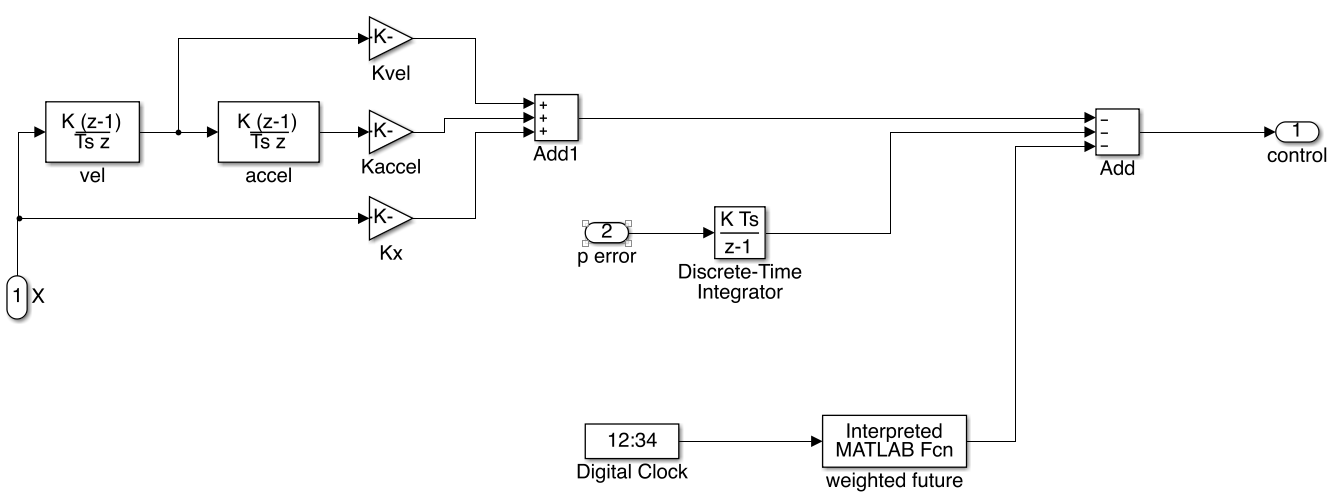
\includegraphics[width=1\textwidth]{18}}
					\caption{Preview controller design. Here X is input of cart current CoM trajectory, p error is an error between the reference ZMP and the measured ZMP, weighted future is function that computes weighted sum of 16000 next time samples of desired ZMP. Control is a control signal that represents the third time derivative of the cart trajectory. Kvel, Kaccel and Kx are $G_x$ components from eq. (\ref{eq:pc1}). Digital clock element is necessary for addressing future values of ZMP reference signal.}
					\label{fig:18}
					\vspace{-0.1cm}
				\end{figure}
				
				The control signal for preview controller is the third time derivative of trajectory and due to this fact a transition block between controller and cart-table model should be provided. This block is an integrator because integration of control signal gives us exactly the second time derivative (acceleration). Preview control of cart table model is represented in \cref{fig:20}
				
				\begin{figure}[H]
					\vspace{-0.2cm}
					\centering
					{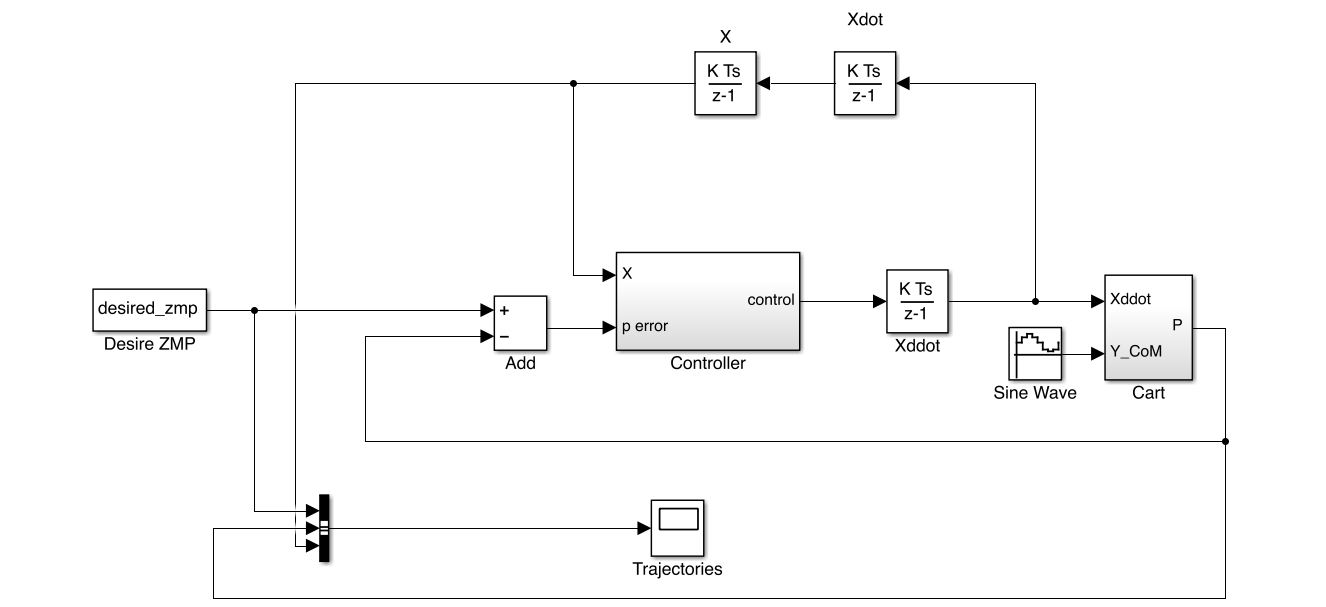
\includegraphics[width=1\textwidth]{20}}
					\caption{Preview control of cart table model.}
					\label{fig:20}
					\vspace{-0.1cm}
				\end{figure}
				
				The results of this controller are represented on \cref{fig:19} and are much better : we can see no late response and no overshooting in ZMP trajectory. Thus the system becomes significantly more stable than in the PID controller case. 
				
				\begin{figure}[H]
					\vspace{-0.2cm}
					\centering
		 			{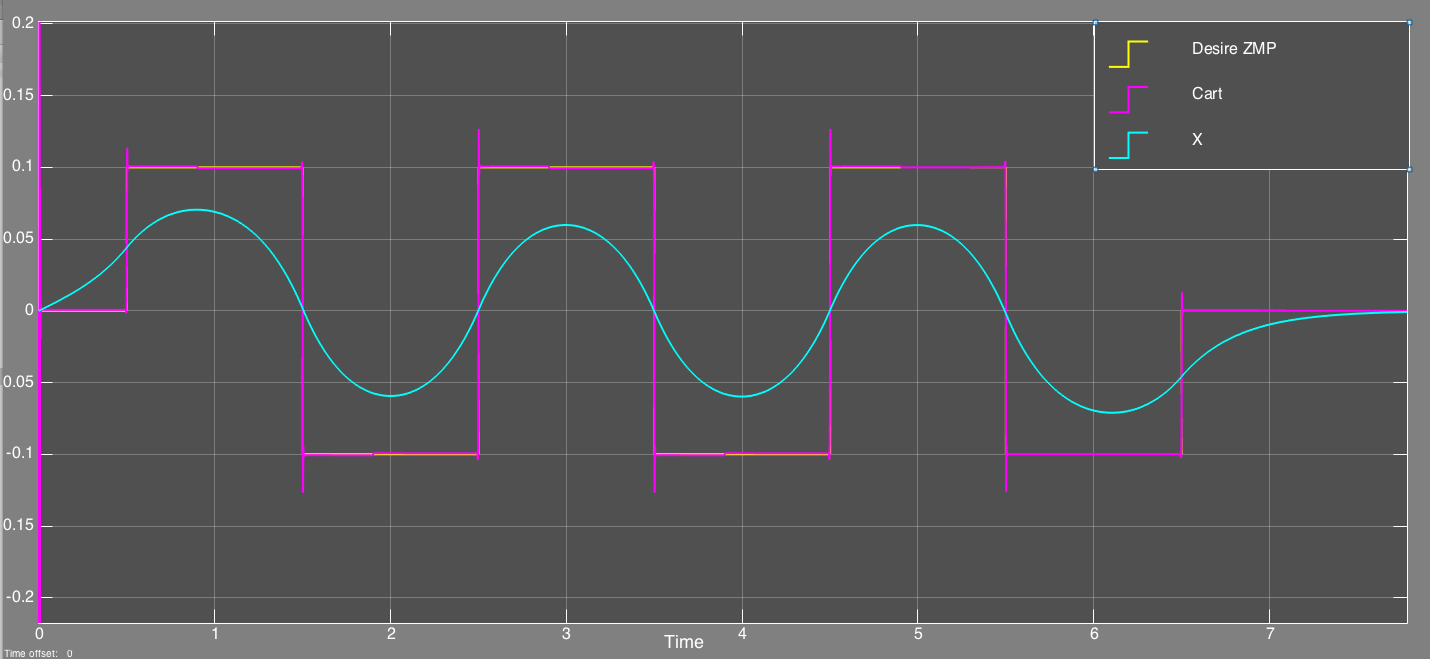
\includegraphics[width=1\textwidth]{19}}
					\caption{Preview controller of cart table model results. Desired ZMP trajectory is yellow and it is not visible due to the fact that actual cart ZMP trajectory that is violet follows ZMP reference signal very well with very little overshoot. Cart CoM trajectory is blue colored.}
					\label{fig:19}
					\vspace{-0.1cm}
				\end{figure}
				
				This developed controller should be applied to the model of robot. Initialy we will consider the simple model of robot.
		\section{Simple Bipedal Robot Model}
			After tuning of preview controller parameters (N samples look ahead) a simple model of a bipedal robot with 12 Degrees of Freedom (DoF) was built. The model is represented on \cref{fig:21}. According to simplification we can write ZMP equation in the following way \cite{ha2007effective}: 
			
			\begin{equation}\label{eq:CoG1}
				\begin{split}
					X_{CoG}(t) = X_{CoG}(0) cosh \left( \sqrt{\dfrac{g}{\alpha Z_{CoG}}} t \right) + \sqrt{\dfrac{\alpha Z_{CoG}}{g}} \dot{X}_{CoG}(0) sinh\left(\sqrt{\dfrac{g}{\alpha Z_{CoG}} } t\right)\\
					Y_{CoG}(t) = Y_{CoG}(0) cosh \left( \sqrt{\dfrac{g}{\beta Z_{CoG}}} t \right) + \sqrt{\dfrac{\beta Z_{CoG}}{g}} \dot{Y}_{CoG}(0) sinh \left( \sqrt{\dfrac{g}{\beta Z_{CoG}}} t \right)
				\end{split}
			\end{equation}
			
			Where $X_{CoG}$, $Y_{CoG}$,  $Z_{CoG}$, $\dot{X}_{CoG}$ and $\dot{Y}_{CoG}$ are X coordinate, Y coordinate, Z coordinate, X velocity and Y velocity of Center of Gravity (CoG) respectively. Parameters $\alpha$ and $\beta$ define robot configuration and the optimal values for our model (\cref{fig:21}) are 0.65 and 0.45 respectively.
			
			\begin{figure}[H]
				\vspace{-0.2cm}
				\centering
				{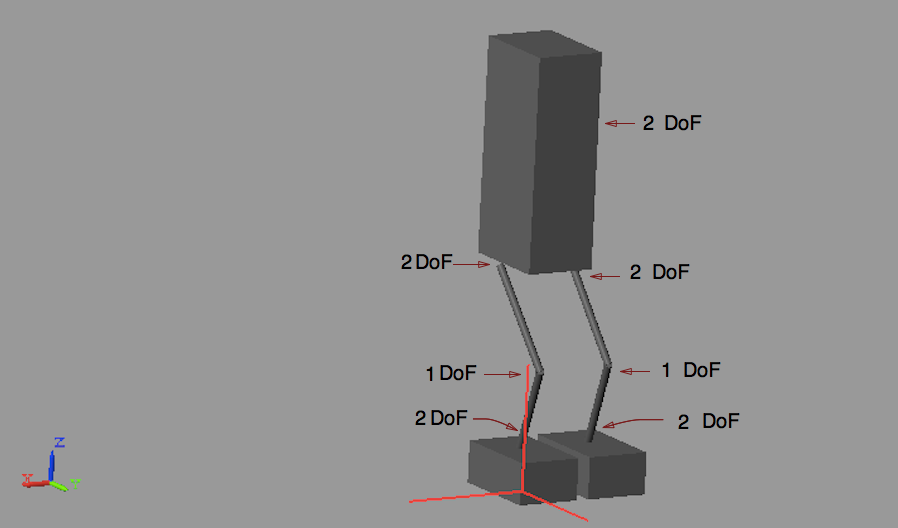
\includegraphics[width=0.7\textwidth]{21}}
				\caption{12 DoF bipedal robot model}
				\label{fig:21}
				\vspace{-0.1cm}
			\end{figure}
			
			Analytical solution of eq. (\ref{eq:eqv1}) applied to bipedal robot with provided $\alpha$ and $\beta$ under the assumption that height of robot's CoM isn't changing significantly can be defined as follows:
			
			\begin{equation}
				X_{CoM} = C_1 e^{-\omega t} + C_2 e^{\omega t}
			\end{equation}
			
			where $C_1 = \dfrac{0.2(1+e^{0.5\omega })}{(e^{-0.5\omega }-e^{0.5\omega })}$, $C_2=-0.2-C_1$, $\omega = \sqrt{\dfrac{g}{Z_c}}$, g is the gravitational acceleration, $Z_c$ is robot's CoM height.
			
			The trajectory of CoM in frontal plane of this analytical solution is represented in \cref{fig:24}.
			
			\begin{figure}[H]
				\vspace{-0.2cm}
				\centering
				{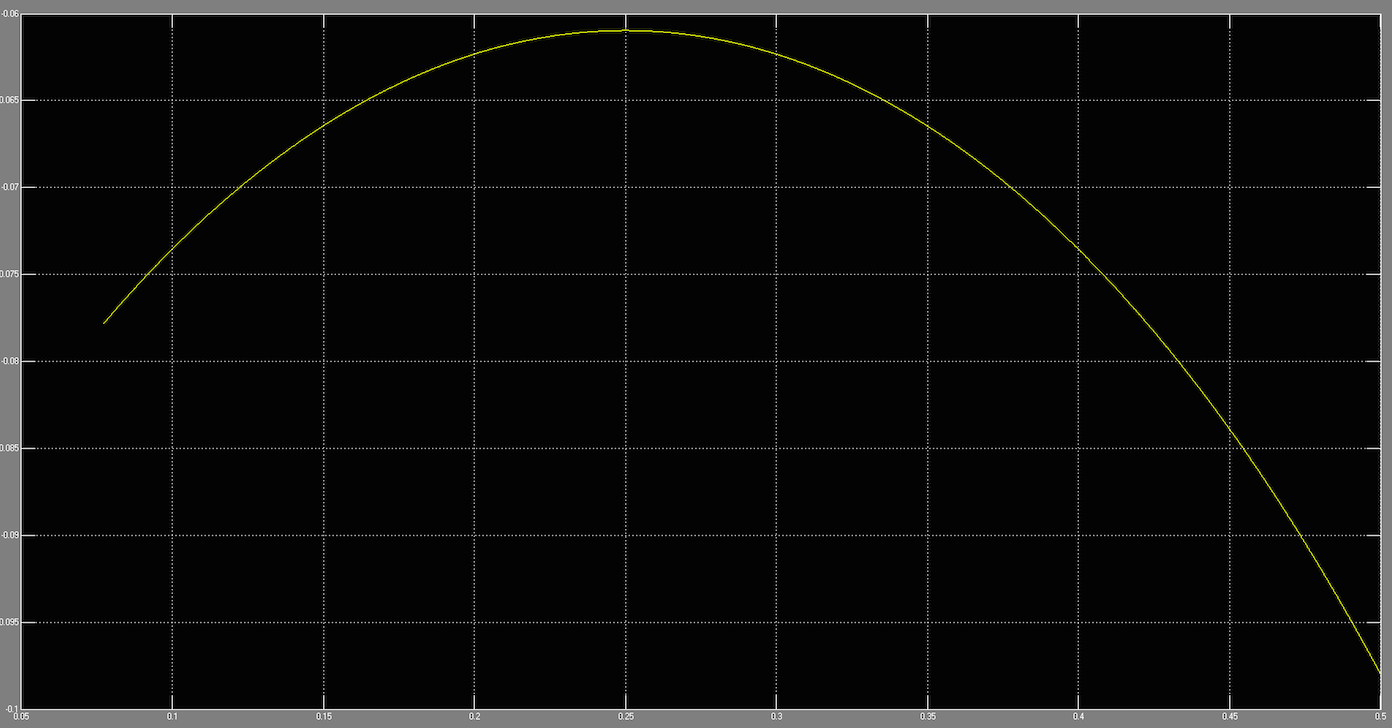
\includegraphics[width=1\textwidth]{24}}
				\caption{Analytically synthesized CoM trajectory.}
				\label{fig:24}
				\vspace{-0.1cm}
			\end{figure}
			
			We can see a very smooth trajectory in \cref{fig:24}. Hence the parameters $\alpha$ and $\beta$ from eq. (\ref{eq:CoG1}) were chosen correctly. 
			
			A direct application of a preview controller shows results which are represented in \cref{fig:25}.
			
			\begin{figure}[H]
				\vspace{-0.2cm}
				\centering
				{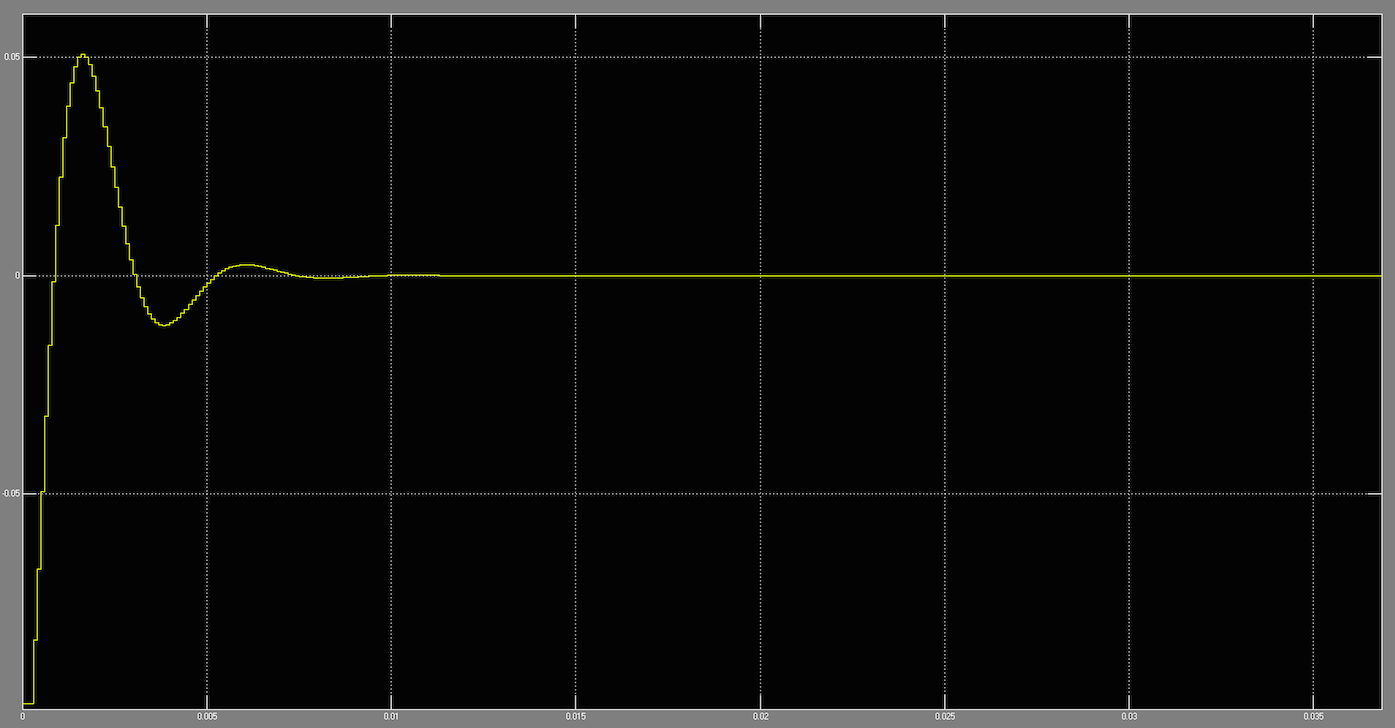
\includegraphics[width=1\textwidth]{25}}
				\caption{Preview control generated CoM trajectory without restriction.}
				\label{fig:25}
				\vspace{-0.1cm}
			\end{figure}
			
			Unfortunately, these results cannot be used in practice because physical motors cannot provide the desired accelerations. We can see a very fast oscillations in the beginning of the trajectory that cannot be performed with physical motors. Hence the preview controller was restricted with maximum motors acceleration.\\
		
			Furthermore, considering the preview control application for CoM trajectory generation in frontal plane it is necessary to mention that some related works, for example \cite{choi2006fuzzy} suggest the use of control signal in the form of eq. (\ref{eq:pc4}) instead of eq. (\ref{eq:pc1}).
			
			\begin{equation}\label{eq:pc4}
				u(k) = -G_I e(i) - G_xx(k) - \sum^{N_l}_{l=1}G_d(l)y_d(k+l)
			\end{equation}
			
			The equation \ref{eq:pc4} has the same meaning as eq. (\ref{eq:pc1}) but it takes the current error e(i) instead of the integral error e(i). There is wasn't found motivation for this form mentioned in articles, but it is obvious that for small disturbances integrated error and current error are small and close to zero. Preview controllers of two forms \ref{eq:pc1} and \ref{eq:pc4} were applied with restrictions to the robot model to generate CoM trajectory in frontal plane. Results are demonstrated in \cref{fig:22}.

		 	\begin{figure}[H]
		 		\vspace{-0.2cm}
		 		\centering
		 		{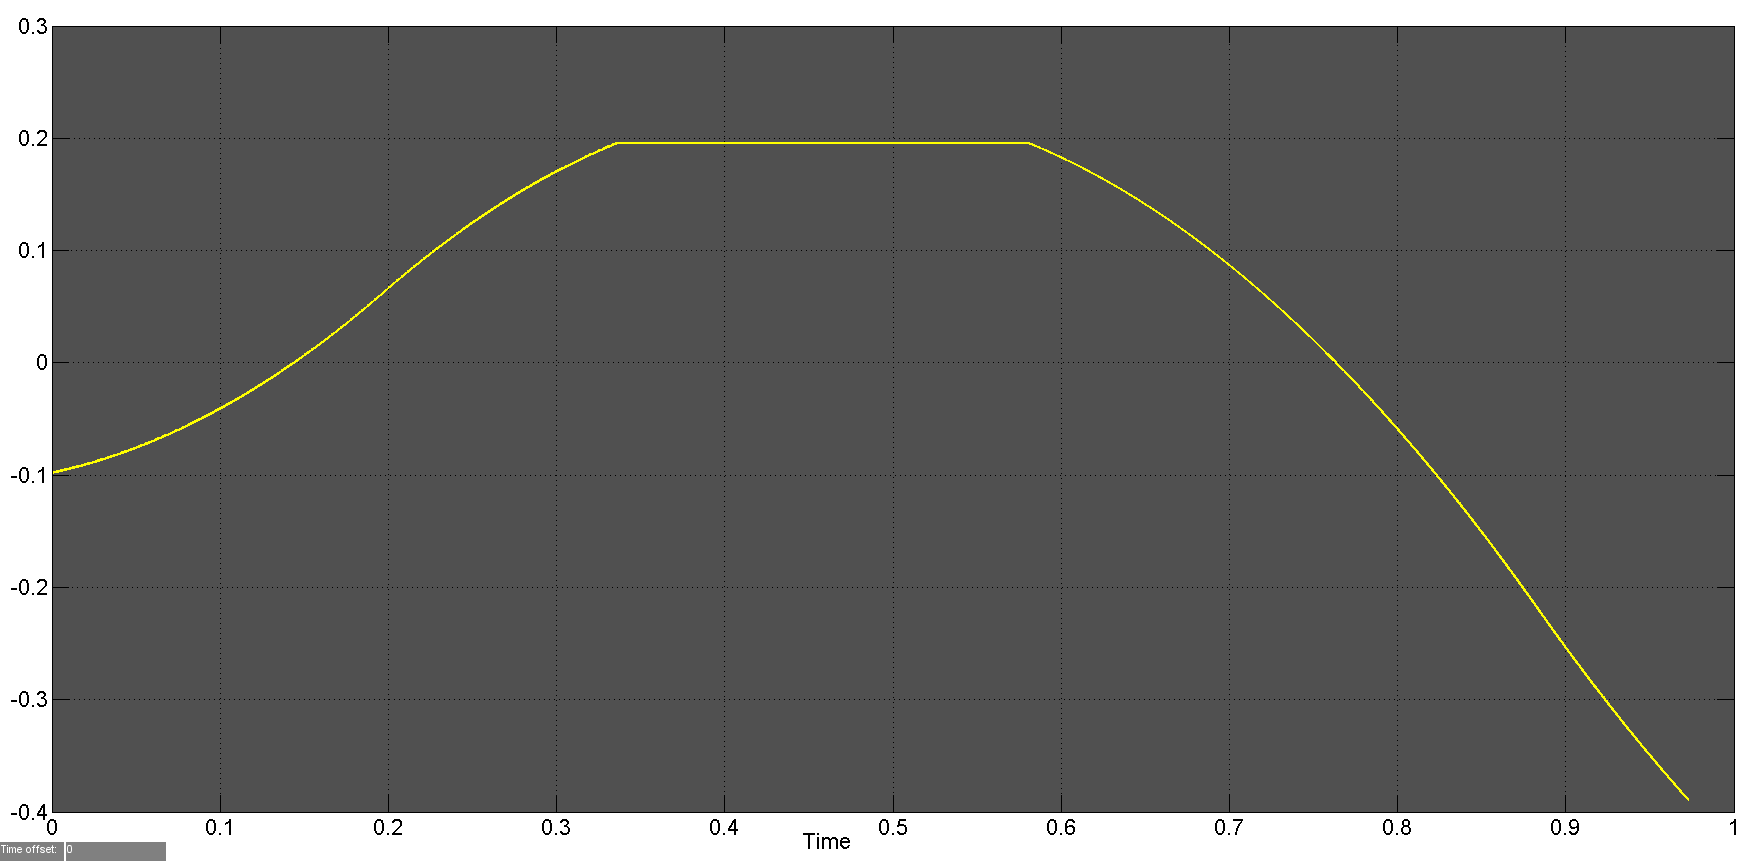
\includegraphics[width=1\textwidth]{22}}
		 		\caption{CoM trajectory in frontal plane generated by the controller which is described by eq. (\ref{eq:pc4})}
		 		\label{fig:22}
		 		\vspace{-0.1cm}
		 	\end{figure}
		 	
		 	We observe in \cref{fig:22} the trajectory that is quite smooth but restricted by the limit.
		 	
		 	\begin{figure}[H]
		 		\vspace{-0.2cm}
		 		\centering
		 		{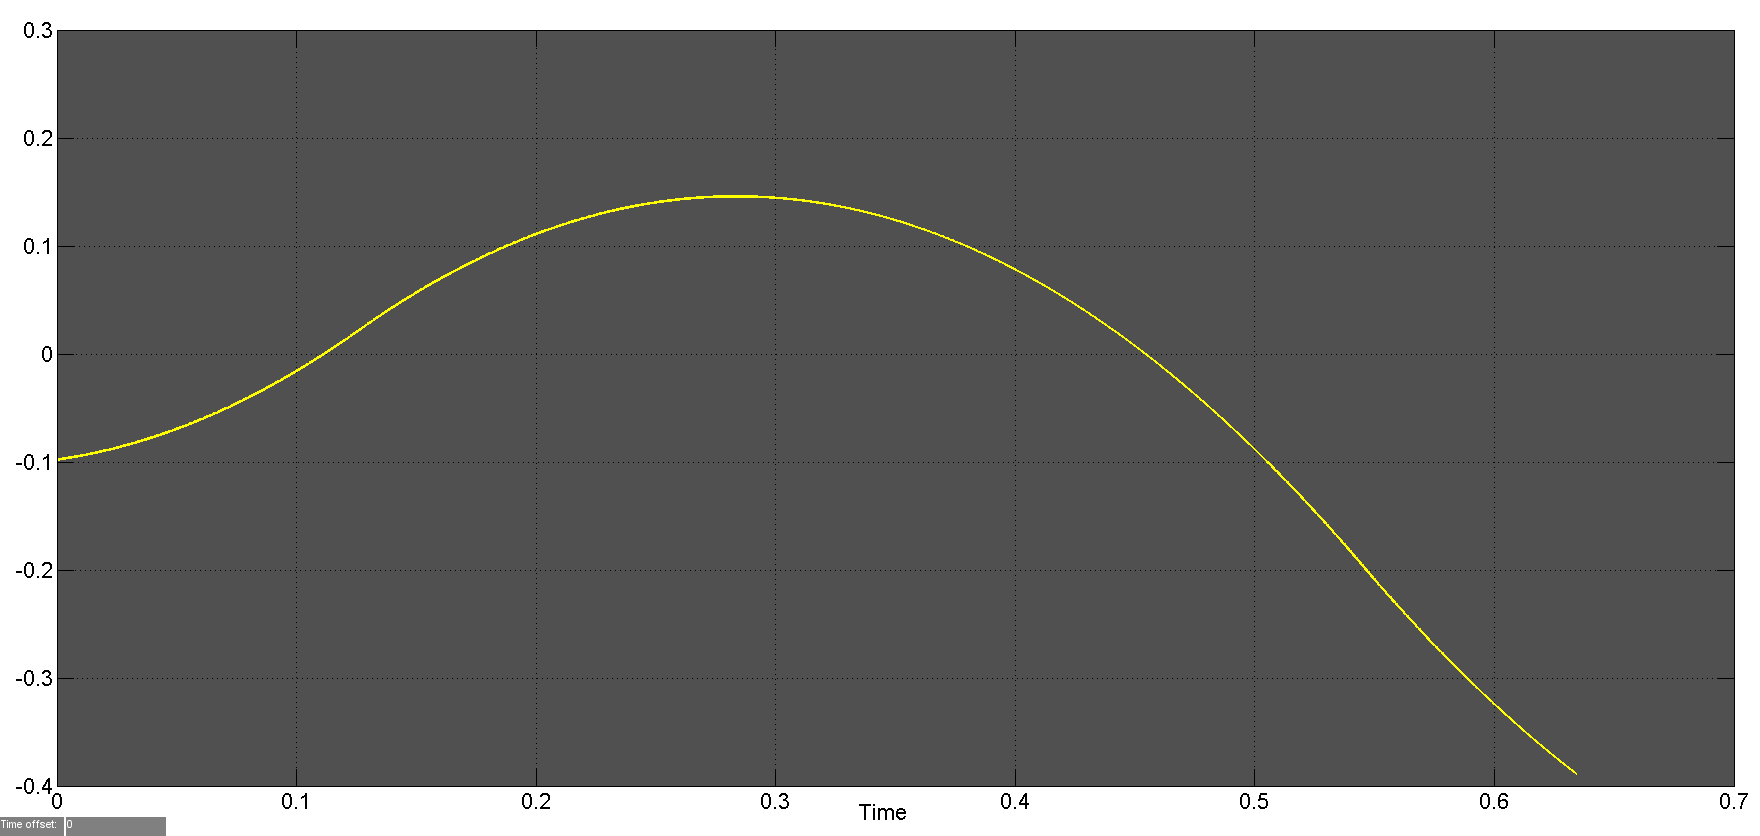
\includegraphics[width=1\textwidth]{23}}
		 		\caption{CoM  Trajectory in frontal plane generated by controller described by eq. (\ref{eq:pc1})}
		 		\label{fig:23}
		 		\vspace{-0.1cm}
		 	\end{figure}
		 	
		 	We see that trajectory depicted in \cref{fig:23} is smoother than trajectory in \cref{fig:22}. Which means that there will be less disturbances provided by the real motors if apply the controller described by equation \ref{eq:pc1}. Hence the controller in the form of eq. (\ref{eq:pc1}) is more preferable than the controller in the form of eq. (\ref{eq:pc4}).
		 	Moreover we see that the trajectory of the analytical derivations is close to the preview controller trajectory. It means that the preview controller can efficiently solve the problem of trajectory generation. This approach is more preferable because it allows a robot to operate in environments with uncertainty because of feedback loop.
	\chapter{Future Work}
		Due to the limitations of the model it is necessary to develop a model that is more similar to a real robot. Moreover to apply the preview controller on a real robot and even on advanced simulator it is still necessary to develop an inverse kinematics module that will transform CoM trajectories to trajectories for every joint. Here a rule based approaches can be used because the robot is a redundant construction and for every trajectory there will be a lot of configurations and thus it is necessary to choose the best one. Moreover it is necessary to combine two controllers in sagital and frontal planes.
		The next step after tuning control parameters on the model is to apply it to a real robot.
		Described in this thesis control method is capable for pattern generation and so future work should consider optimization methods for generated trajectory to prevent the robot from falling on the rough terrain.
		When control algorithm is developed the structure of the robot should be revised in order to maintain optimal criteria. For example this criteria could be an energy consumption or the speed of the movements.
		After several iterations of algorithm and structure optimization the robot will become able for walk, however further investigations of AI and object detection are still necessary. It is reasoned by the level of autonomy that we want robot to achieve. It is impossible to preprogram all the possible conditions for the robot and hence it have to deal with some level of uncertainty.
	\chapter{Summary}
		In this work different approaches to bipedal locomotion were considered. Classification of existing methods was also done and it was the basics for development of a dynamic balance algorithm for bipedal robot locomotion. Two approaches were chosen: analytical one (ZMP criteria for dynamical stability) and CPG (controller output should generate a pattern for locomotion). Results of implemented preview controller on provided models show stable smooth trajectories and thus it seems reliable to try this approach on the real robot. There are works \cite{kajita2003biped, audren2014model} that already applied preview controller to real robots. However in their works the authors don't consider application of these techniques to simulation of the robot and don't provide technical details. As shown in Chapter 4 a direct application of preview controller to robot model gives very good but physically unreachable results. Due to the fact that motors have limited accelerations, the system cannot react as fast as the controller tries to stabilize the system. The controller was limited by the constraints of the physical motors and the results of control became similar to the fully analytical solution during one step period. Hence the developed approach is promising because it can adapt to disturbances and uneven terrain because of feedback loop.
		Moreover stable bipedal locomotion requires efficient processing of sensors data in order to predict possible disturbances before they are applied to the robot.
			
	\bibliographystyle{unsrtnat}
	\bibliography{robotics}
	
	\begin{appendices}
		\chapter{Preview control parameters estimation algorithm}
			\begin{lstlisting}
% compute preview controller coefficients
function [Ke, Kx, G] = preview_control_params(T, Zh, N)
	% Cost function optimisation parameters
	R = 1e-6; 
	Qe = 1;
	Qdpos = 0;
	Qdvel = 0;
	Qdaccel = 0;
	
	g = 9.8; % gravity acceleration
	
	% derivative state coefficient matrix
	A = [1 T T^2/2;0 1  T;0 0 1];
	B = [T^3/6;T^2/2;T];
	% coefficient matrix of state space model
	C = [1 0 -Zh/g];
	
	% constructing matrices for DARE
	AA = vertcat(horzcat([1], C*A),horzcat(zeros(3,1), A));
	BB = vertcat([C*B], [B]);
	RR = R;
	QQ = diag([Qe, Qdpos, Qdvel, Qdaccel]);
	
	% DARE equation solving
	PP = dare(AA,BB,QQ,RR);
	
	SS = 1.0/(RR + BB'*PP*BB);
	KK = SS*BB'*PP*AA;
	
	% coefficients for regulator
	Ke = KK(1,1);
	Kx = KK(1,2:4);
	
	Ac = AA - BB*KK;
	XX = -Ac' * PP * [1,0,0,0]';
	
	% first preview coefficient should be equal -Ke
	G = [-Ke];
	
	% compute preview coefficients
	for i=2:1:N
		G = [G SS * BB' * XX];
		XX = Ac' * XX;
	end
end
			\end{lstlisting}
		\chapter{Desired ZMP generation algorithm}
			\begin{lstlisting}
g = 9.8; % gravity acceleration
Zc = 0.85; % height of CoM
T = 1e-4; % descitisation step
N = 16000; % preview steps
sim_time = 10; % simulation time

% compute control coefficients
[Ke, Kx, G] = preview_control_params(T, Zc, N);

D_o = [1 3 5]';                     % delays
D_e = [2 4 6]';                     % delays
t = 0 : T : sim_time + N * T;  % signal evaluation time
width = 1;                            % width of each pulse

% desired ZMP signal construction
desired_zmp = 0.1 * pulstran(t, D_o, 'rectpuls', width)\
- 0.1 * pulstran(t, D_e, 'rectpuls', width);
% convert desired ZMP to simulink signal format
desired_zmp = [t' desired_zmp'];
			\end{lstlisting}
	\end{appendices}
  
\end{document}